% Beamer Presentation
% LaTeX Template
% Version 1.0 (10/11/12)
%
% This template has been downloaded from:
% http://www.LaTeXTemplates.com
%
% License:
% CC BY-NC-SA 3.0 (http://creativecommons.org/licenses/by-nc-sa/3.0/)
%

%----------------------------------------------------------------------------------------
%	PACKAGES AND THEMES
%----------------------------------------------------------------------------------------

\documentclass[usenames,dvipsnames]{beamer}

\mode<presentation> {

% The Beamer class comes with a number of default slide themes
% which change the colors and layouts of slides. Below this is a list
% of all the themes, uncomment each in turn to see what they look like.

%\usetheme{default}
% \usetheme{AnnArbor}
%\usetheme{Antibes}
%\usetheme{Bergen}
% \usetheme{Berkeley}
% \usetheme{Berlin}
%\usetheme{Boadilla}
%\usetheme{CambridgeUS}
% \usetheme{Copenhagen}
\usetheme{Darmstadt}
% \usetheme{Dresden}
% \usetheme{Frankfurt}
% \usetheme{Goettingen}
%\usetheme{Hannover}
%\usetheme{Ilmenau}
%\usetheme{JuanLesPins}
%\usetheme{Luebeck}
% \usetheme{Madrid}
% \usetheme{Malmoe}
%\usetheme{Marburg}
% \usetheme{Montpellier}
% \usetheme{PaloAlto}
% \usetheme{Pittsburgh}
%\usetheme{Rochester}
% \usetheme{Singapore}
%\usetheme{Szeged}
%\usetheme{Warsaw}

% As well as themes, the Beamer class has a number of color themes
% for any slide theme. Uncomment each of these in turn to see how it
% changes the colors of your current slide theme.

% \usecolortheme{albatross}
%\usecolortheme{beaver}
%\usecolortheme{beetle}
%\usecolortheme{crane}
%\usecolortheme{dolphin}
%\usecolortheme{dove}
%\usecolortheme{fly}
\usecolortheme{lily}
%\usecolortheme{orchid}
%\usecolortheme{rose}
%\usecolortheme{seagull}
%\usecolortheme{seahorse}
%\usecolortheme{whale}
%\usecolortheme{wolverine}

%\setbeamertemplate{footline} % To remove the footer line in all slides uncomment this line
%\setbeamertemplate{footline}[page number] % To replace the footer line in all slides with a simple slide count uncomment this line

\setbeamertemplate{navigation symbols}{} % To remove the navigation symbols from the bottom of all slides uncomment this line
}

% % -------------------------------------------
% % Songkai added, feel free to delete --------
% \AtBeginSection[]{
%   \begin{frame}
%   \vfill
%   \centering
%   \begin{beamercolorbox}[sep=8pt,center,shadow=false,rounded=true]{title}
%     \usebeamerfont{title}\insertsectionhead\par%
%   \end{beamercolorbox}
%   \vfill
%   \end{frame}
% }
% % Songkai added, feel free to delete --------
% % -------------------------------------------




\usepackage{graphicx} % Allows including images
\usepackage{booktabs} % Allows the use of \toprule, \midrule and \bottomrule in tables
\usepackage{natbib}
\usepackage{amsmath, amssymb, graphicx, url}
\usepackage[ruled]{algorithm2e}
\usepackage{commath}
\usefonttheme[onlymath]{serif}

\usepackage{amsmath}
\usepackage{amssymb}
\usepackage{centernot}
%\usepackage[a4paper, margin=0.8in]{geometry}
\usepackage{parskip}
\usepackage{graphicx}

\usepackage{natbib}

\usepackage{tikz}
\usepackage{tikzlings}

\usepackage{tabularx}
\usepackage{array}
\usepackage{multirow}
\usepackage{makecell}
\usepackage{mathtools}
\usepackage{bm,upgreek}
\usepackage{subcaption}
\usepackage{textpos}
% \usepackage{eso-pic}

% \usepackage{multimedia}
\usepackage{media9}

\def\E{\mathbf{E}}
\def\PP{\mathbf{P}}
\def\Reals{\mathbb{R}}
\def\Naturals{\mathbb{N}}
\def\argmin{\operatornamewithlimits{arg\,min}}
\def\deq{:=}
\def\wh#1{\widehat{#1}}
\def\bd#1{\mathbf{#1}}
\def\bx{\bd{x}}
\def\by{\bd{y}}
\def\bZ{\bd{Z}}
\def\bB{\bd{B}}
\def\bV{\bd{V}}
\def\tO{{\tilde{\cO}}}
\def\tOm{\tilde{\Omega}}
\def\barw{\overline{w}}
\def\d{{\mathrm d}}
\def\ave#1{\langle #1 \rangle}
\def\Ave#1{\left\langle #1 \right\rangle}
\def\eps{\varepsilon}
\def\tr{\mathrm{Tr}}


\def\HS{\mathbb{H}}
\def\reals{\mathbb{R}}
\def\ths{\theta^*}
\def\thh{\hat{\theta}}
\def\lbr{\left[}
\def\rbr{\right]}
\def\lc{\left(}
\def\rc{\right)}


    \def\ddefloop#1{\ifx\ddefloop#1\else\ddef{#1}\expandafter\ddefloop\fi}
    % \cA, \cB, ...
    \def\ddef#1{\expandafter\def\csname c#1\endcsname{\ensuremath{\mathcal{#1}}}}
    \ddefloop ABCDEFGHIJKLMNOPQRSTUVWXYZ\ddefloop
    \def\argmin{\operatornamewithlimits{arg\,min}}
    \def\E{\mathbf{E}}
    \def\bx{\bd{x}}
	\def\by{\bd{y}}
    \def\bZ{\bd{Z}}

\newcommand{\propnumber}{} % initialize
\newtheorem*{prop}{Proposition \propnumber}
\newenvironment{propc}[1]
  {\renewcommand{\propnumber}{#1}%
   \begin{shaded}\begin{prop}}
  {\end{prop}\end{shaded}}

\newcommand{\crlrnumber}{} % initialize
%\newtheorem*{corollary}{Corollary \crlrnumber}
\newenvironment{corollaryc}[1]
  {\renewcommand{\crlrnumber}{#1}%
   \begin{shaded}\begin{corollary}}
  {\end{corollary}\end{shaded}}

\theoremstyle{definition}
% \newtheorem{definition}




% \setbeamertemplate{headline}{% 
%     \leavevmode%
%     \hbox{%
%         \begin{beamercolorbox}[wd=.4\paperwidth,ht=2.25ex,dp=1ex,right]{section in head/foot}%
%             \usebeamerfont{section in head/foot}\insertshorttitle\hspace*{2ex}
%         \end{beamercolorbox}%
%         \begin{beamercolorbox}[wd=.6\paperwidth,ht=2.25ex,dp=1ex,left]{subsection in head/foot}%
%             \usebeamerfont{section in head/foot}
\includegraphics[height=2ex,keepaspectratio]{Slides/Block_M-Hex.png}\hspace*{2ex}\insertsectionhead
%         \end{beamercolorbox}%
%     }
% }

% \addtobeamertemplate{headline}{}{%
% \begin{textblock*}{100mm}(.85\textwidth,-1cm)
% \Huge\textcolor{white}{\textbf{\TeX}}
% \end{textblock*}}



%----------------------------------------------------------------------------------------
%	TITLE PAGE
%----------------------------------------------------------------------------------------

%%%% TRY WITH TEXTPOS
% \newcommand{\imgblock}{\begin{textblock*}{5cm}(10.5cm,-1.2cm) % {block width} (coords)
%         
\includegraphics[width=1cm]{Slides/Block_M-Hex.png} % loading the image
%     \end{textblock*}
%     }

% \addtobeamertemplate{background}{\imgblock}{}



% \setbeamertemplate{headline}{\hfill
\includegraphics[width=1.5cm]{Slides/Block_M-Hex.png}\hspace{0.2cm}\vspace{-1cm}}

% \logo{
\includegraphics[height=1cm]{Slides/Block_M-Hex.png}}

\addtobeamertemplate{frametitle}{}{%
    \begin{textblock*}{5cm}(10.5cm, -0.8cm)
        
\includegraphics[width=0.9cm]{Block_M-Hex.png} % your logo file here
    \end{textblock*}
}

\definecolor{mycolor}{cmyk}{100, 60, 0, 60}
\definecolor{my_maize}{rgb}{0.9608,0.7137,0.2588}
\definecolor{my_yellow}{rgb}{0.9294,0.8196,0.2706}

% \setbeamercolor{section in head/foot}{fg=cyan}
\setbeamercolor{section in head/foot}{fg=my_maize}

\setbeamercolor{frametitle}{bg=mycolor}
\setbeamercolor{titlelike}{fg=black, bg=yellow}

\usepackage{url}
\usepackage{hyperref}

\usepackage{xcolor}

\hypersetup{pdfauthor={Name},
            colorlinks=true,
            linkcolor={my_yellow},
            % citecolor={blue},
            % linkcolor=[RGB]{0.949, 0.784, 0.035}
            }

% fix inconsistent colors in cite parenthesis (where the closing parenthesis were black instead of the rest of the citecolor!)
% https://github.com/josephwright/beamer/issues/671
\let\oldcite=\cite
\let\oldcitet=\citet
\let\oldcitep=\citep 
\renewcommand{\citet}[2][]{\textcolor{green}{\oldcitet[#1]{#2}}}
\renewcommand{\citep}[2][]{\textcolor{green}{\oldcitep[#1]{#2}}}
\renewcommand{\cite}[2][]{\textcolor{green}{\oldcite[#1]{#2}}}
            

\title[Group Meeting]{An Overview of Neural ODEs}
% and Estimation of Predictive Uncertainties
% The short title appears at the bottom of every slide, the full title is only on the title page

\author[Aniket Jivani]{Aniket Jivani}
% \institute[U-M]{University of Michigan}

\date{\today}

\AtBeginSection[]
{
 \begin{frame}<beamer>
 \frametitle{Plan}
 \tableofcontents[currentsection]
 \end{frame}
}


\begin{document}

\begin{frame}
\titlepage % Print the title page as the first slide
\end{frame}



\begin{frame}
 \frametitle{Overview} % Table of contents slide, comment this block out to remove it
 \tableofcontents % Throughout your presentation, if you choose to use \section{} and \subsection{} commands, these will automatically be printed on this slide as an overview of your presentation
\end{frame}

\section{Background}

\begin{frame}{Traditional modeling workflow}

    \begin{figure}
        \centering
        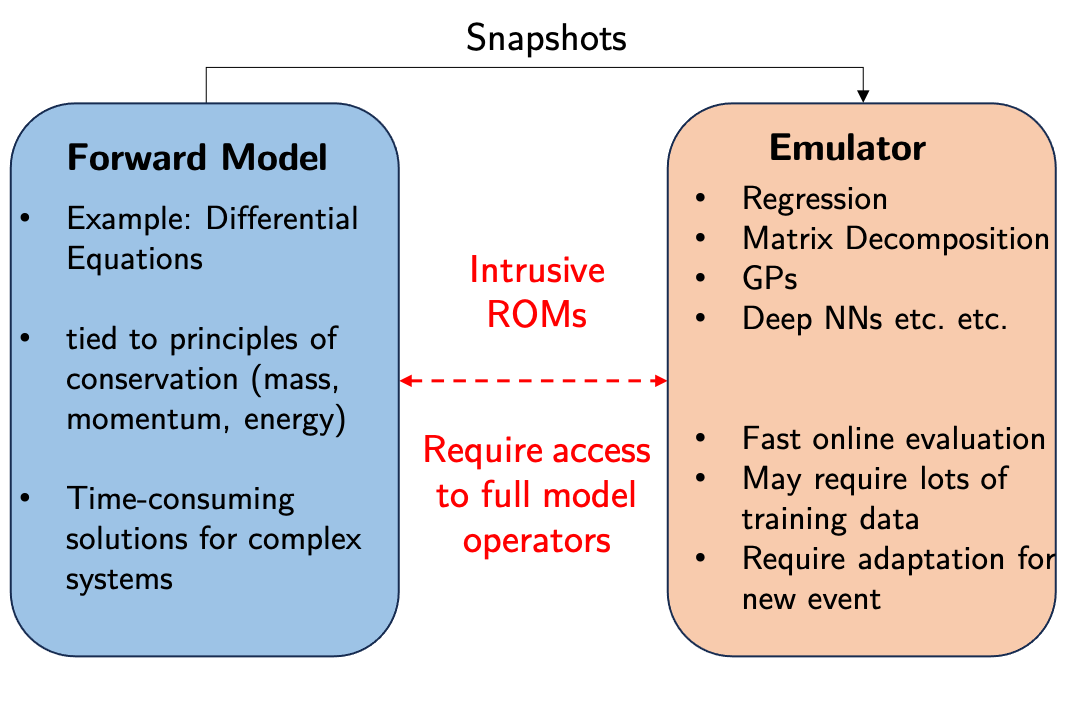
\includegraphics[width=0.7\linewidth]{ModellingDichotomy.png}
        % \caption{Enter Caption}
        \label{fig:fm_emulators}
    \end{figure}

    \textbf{Try: } Combine approaches for more useful and interpretable surrogate models.

    To clarify, not all data we observe lends itself to combining these paradigms naturally or easily.


\end{frame}
% \begin{frame}{Modeling Approaches}
% \begin{itemize}
%     \item Most modeling approaches can be \emph{loosely} classified as mechanistic and non-mechanistic

%     \item Mechanistic: Define laws governing the underlying phenomenon - cellular automata, PDEs, etc. Generalizable, do not need to consume huge datasets to provide a solution (closed-form or otherwise).

%     \item Need constant improvement and introduction of new physics to account for mismatch with reality

%     \pause

%     \item Non mechanistic models: so-called `black boxes'. Fit empirical relations, surrogate models, model selection. Can guide design of mechanistic models.

%     \item We usually have an iterative loop between these two.
% \end{itemize}
% \end{frame}

% \begin{frame}{approximations}
%     Mechanistic to non-mechanistic - non-intrusive: reduce offline training costs
%     intrusive - plug expansions back into original models, solve a system of equations

%     What we look for: hybrid methods: incorporate some constraints on the surrogate model, faster surrogate building time, enable UQ
% \end{frame}

% \begin{frame}{Foxes and Rabbits}
%     \begin{quote}
%         Since Newton, mankind has come to realize that the laws of physics are always expressed in the language of differential equations - Steven Strogatz
%     \end{quote}

%     show applications - biology, epidemiology, reliability analysis
% \end{frame}




% \begin{frame}{Seeking solutions to PDEs}
% \begin{itemize}
%     \item Most common approach: Convert to a system of ODEs (LeVeque) via the so-called Method of Lines

%     \item Initial value problems vs Boundary value problems - typically prefer the former (Reasons? easy to show existence and uniqueness, though a rise of approaches that go the other way too!)

%     \item Solution methods: Various families of solvers that do one or multi-step updates: Show Runge-Kutta, explain NFE etc.
% \end{itemize}

% \textcolor{red}{To DO}
% Show ``spectrum'' of approaches on a line: purely black-box mappings (NeurOps, DeepONets - competitors :-)), fully prespecified but by playing around with definitions can be used to ``discover'' the system (PINNs), and the middle ground (deep equilibrium models, SINDy and Operator Inference, implicit layer models like SIREN, Neural ODEs, flow maps paper by Churchill and Xiu)
% It is worth mentioning that while these two are useful in their own right, the discretization invariance is still a huge advantage of NOps which is a hurdle for these other methods.

% Show unanswered questions as scatter points around the keyword on the line. UQ? Latent parameter mappings? Transferability? Predictive uncertainties? More general open questions - making these more data efficient processes? 

% \end{frame}

\begin{frame}{Building more useful surrogate models}
(fuzzy classification, arguably flow maps also belong on left.)


\begin{figure}
    \centering
    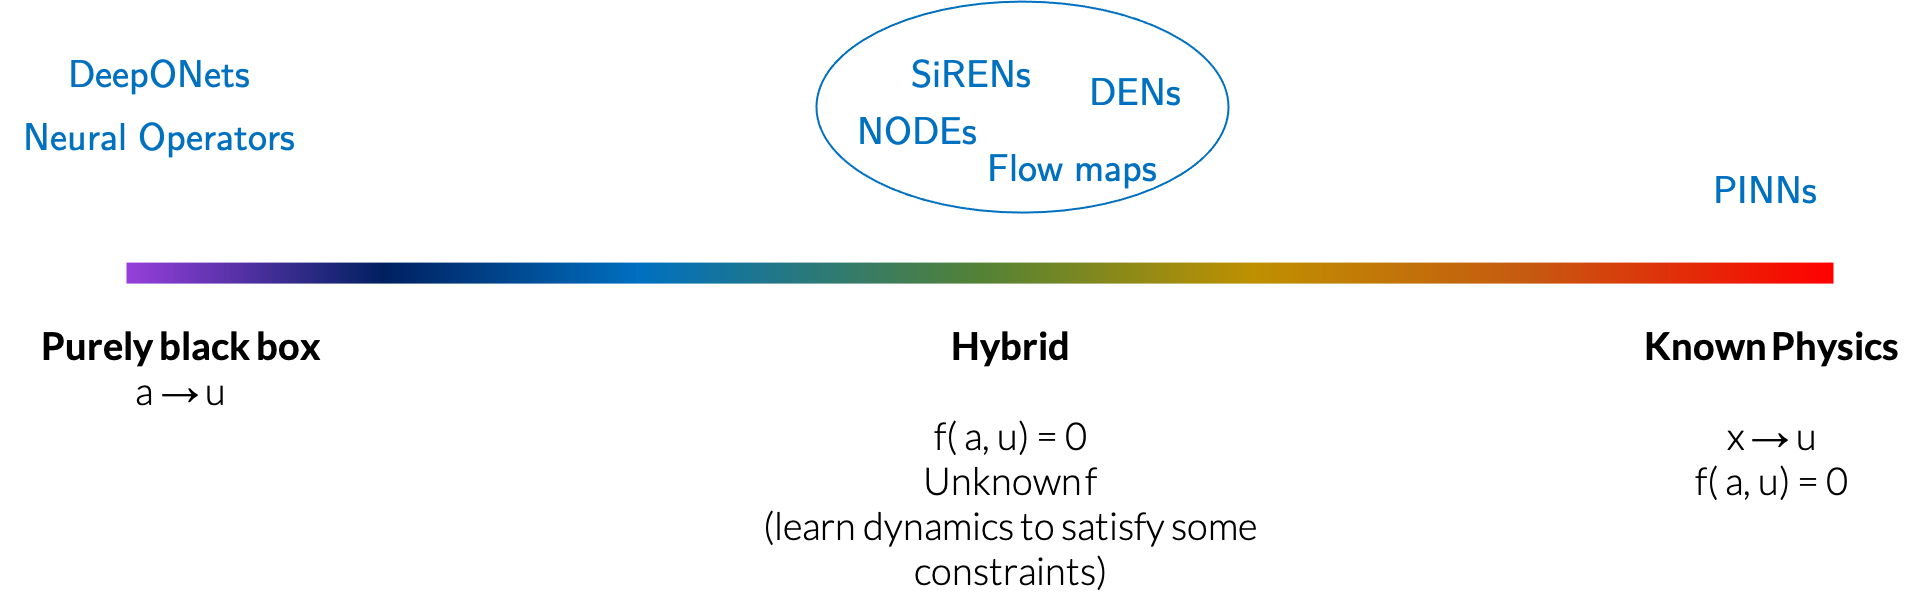
\includegraphics[width=0.95\linewidth]{SpectrumOfPDESolvingApproaches.png}
    % \caption{Enter Caption}
    \label{fig:spectrum_pde}
\end{figure}

% \begin{tikzpicture}
%     \elephant[3D]
% \end{tikzpicture}

Interesting Questions:
\begin{enumerate}
    \item Quantifying uncertainties when extrapolating in small data regime (1D and above)

    \item Jointly modeling state and latent parameters

    \item Inference on partial inputs
\end{enumerate}

\end{frame}

\begin{frame}{Brief detour: PINNs}
  \cite{Raissi2019} \href{www.sciencedirect.com/science/article/pii/S0021999118307125}{(...see full text here)}: 
    $u_t+\mathcal{N}[u]=0, \, x\in\Omega, \, t\in[0,T]$

    $f = u_t+\mathcal{N}[u]$

    $MSE=MSE_u+MSE_f$

    where $MSE_u=\frac{1}{N_u}\sum_{i=1}^{N_u}|u(t_u^i,x_u^i)-u^i|^2$

    and $\quad MSE_f=\frac{1}{N_f}\sum_{i=1}^{N_f}|f(t_f^i,x_f^i)|^2$

    Here, \textcolor{red}{$\left\{t_{u}^{i},x_{u}^{i},u^{i}\right\}_{i=1}^{N_{u}}$} are initial and boundary training data on $u(t, x)$ and 

    \textcolor{red}{$\left\{t_{f}^{i},x_{f}^{i}\right\}_{i=1}^{N_{f}}$} specify collocation points for $f(t, x)$.

    \textbf{Drawback: } In high-D problems, lots of collocation points to globally enforce physics-informed constraint. (costly, slow training)
\end{frame}

\begin{frame}{Extensions}
    Also don't do well with \emph{PDE systems whose behavior has sharp gradients (e.g., propagating fronts of waves) or complex
    local morphology. } \cite{ren_phycrnet:_2022}

    \cite{sun_surrogate_2020} \emph{...if ICs and BCs are well imposed thus the corresponding PDE problem is well-defined, in principle, the unique solution should be captured by the DNN via PDE-constrained learning without any labeled data}

    Approach 1: Split into particular solution for boundaries and weighted solution for interiors (\textcolor{red}{$D(t, \mathbf{x}, \theta)$ is zero on boundaries and increases away from it.})

    $$\begin{aligned}\hat{\mathbf{u}}(t,\mathbf{x},\boldsymbol{\theta};\mathbf{W},\mathbf{b})&=\mathbf{u}_{par}(t,\mathbf{x},\boldsymbol{\theta})+D(t,\mathbf{x},\boldsymbol{\theta})\tilde{\mathbf{u}}(t,\mathbf{x},\boldsymbol{\theta};\mathbf{W},\mathbf{b})\\\hat{p}(t,\mathbf{x},\boldsymbol{\theta};\mathbf{W},\mathbf{b})&=p_{par}(t,\mathbf{x},\boldsymbol{\theta})+D(t,\mathbf{x},\boldsymbol{\theta})\tilde{\boldsymbol{p}}(t,\mathbf{x},\boldsymbol{\theta};\mathbf{W},\mathbf{b})\end{aligned}$$
\end{frame}

\begin{frame}{Extensions (contd.)}
    Approach 2: Constraints in the architecture...\cite{gao_phygeonet:_2021}
    \begin{figure}
        \centering
        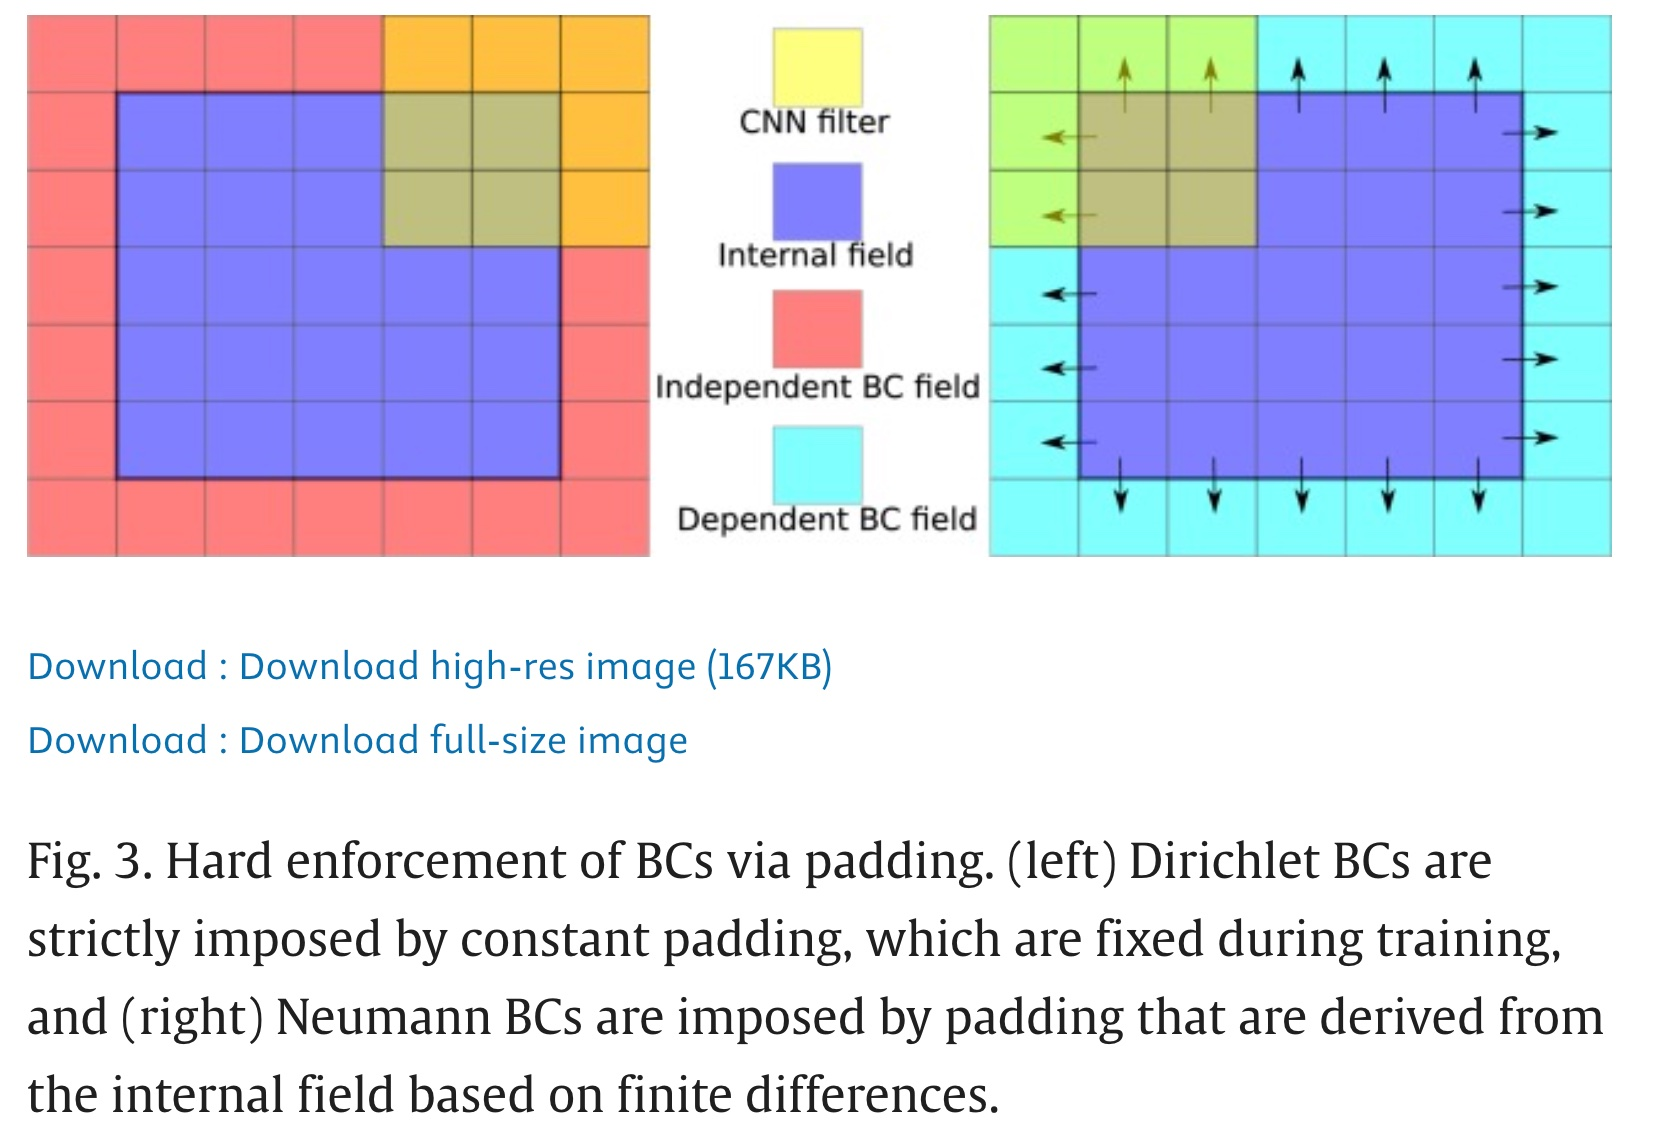
\includegraphics[width=0.8\linewidth]{HardCodedBCsCNN.jpg}
        % \caption{Enter Caption}
        \label{fig:bc_cnn}
    \end{figure}

    Now back to the topic at hand!
\end{frame}

% \begin{frame}{IVP vs BVP}
% \begin{itemize}
%     \item Not an expert, but a quick look at the literature and the theory suggests its easier most of the time to do IVPs (\emph{practically method of lines vs method of lines transposed})

%     \item See page 38 of \href{www.tevza.org/home/course/modelling-II_2016/books/Leveque\%20-\%20Finite\%20Difference\%20Methods.pdf}{LeVeque} for a good example. % LaTeX cannot handle percent signs in a URL.
    
%     \item Example of conversion between BVP and IVP

%     \item For BVPs, not all of them have solutions, and when solutions exist, they are not always unique! Some problems can have multiple solutions

%     \item Some recent work trying to leverage BVP / root finding type algorithms for more efficiency.
% \end{itemize}
% \end{frame}

\begin{frame}{Initial Value Problem}
    % Reference: \href{http://tevza.org/home/course/modelling-II_2016/books/Leveque%20-%20Finite%20Difference%20Methods.pdf}{Finite Difference Methods (Leveque)}
    $$\frac{dy}{dt} = f(y(t), t, \textcolor{red}{\mu}) \quad \text{for } t > t_0$$

    with initial condition (IC) $y(t_0) = y_0$. $\mu$ represents a parametrized system (which we will use). $y$ is the response or state variable to solve for.

    In general, the above may refer to a system of ODEs where $y = [y_1, \cdots, y_n]$. Alternately: $\dot{x} = f(x, t)$, $y = h(x, t)$ where $y$ is the QoI.
    
    \textbf{Linear:} $f(y, t) = A(t)y + g(t)$ (express as $Ly=f$ where $L$ is linear)
    
    \textbf{Constant Coefficient:} $A(t)=A$ - can define a closed form solution
    
    \emph{General case:} No closed form solution, need integrators.
\end{frame}

% \begin{frame}{Existence and Uniqueness}
    % Existence and uniqueness is guaranteed if $f$ is continuous on a region containing $t_0$ and is Lipschitz continuous w.r.t. $y$ i.e.

    % $|f(y_1) - f(y_2)| \leq K |y_1 - y_2|$
% \end{frame}


\begin{frame}{ODE Solvers}
    % Lots of literature here, but for our purposes we will just look at commonly used methods for  \href{https://en.wikipedia.org/wiki/Stiff_equation}{non-stiff ODEs}
    % \textcolor{red}{find a better reference for stiffness}
    % \begin{itemize}
    % \end{itemize}
    Example: Runge-Kutta Family of methods, RK4 below:

    $$\begin{aligned}
        &k_{1} =f(y^*(t_0),t_0)  \\
        &k_{2} =f\left(y^*(t_0)+k_1\frac h2,t_0+\frac h2\right)  \\
        &k_{3} =f\left(y^*(t_0)+k_2\frac h2,t_0+\frac h2\right)  \\
        &k_{4} =f\left(y^*(t_0)+k_3h,t_0+h\right) 
    \end{aligned}$$

    \textbf{Update:}$$y^*(t_0+h)=y^*(t_0)+\frac{k_1+2k_2+2k_3+k_4}6h$$

    (typically use solvers with adaptive time-stepping; we will come back to this later)

\end{frame}


% \begin{frame}{Method of Lines Discretizations}
    
% \end{frame}

% \begin{frame}{ROMs}
% \begin{itemize}
%     \item Access to original governing equations - convert to a reduced-order model
    
%     \item Propose intrusive and non-intrusive approaches to get to solution of ROMs
% \end{itemize}
% \end{frame}

% \begin{frame}{Surrogate Models for ODEs}
% \begin{itemize}
%     \item Amongst matrix decomposition methods, POD-type approaches have been around for a long time. Can we use the general framework to tackle ODEs too?

%     \item Yes, nothing in the formulation restricts us. However $\cdots$

%     \item Truncation error affects us more severely in time-dependent systems! Not sufficient by itself to ensure a robust performant mapping.

%     \item Yes, there are non-linear dim reductions approaches too - including an interesting one that uses Wasserstein barycenters to interpolate between solution snapshots. However, we are looking to approximate mapping between $dy/dt$ and $f$ here, so we will not talk about these for now.
% \end{itemize}
% \end{frame}

\section{Methodology}

% \begin{frame}{Explicit Approaches}
% \begin{itemize}
%     \item Operator Inference, SINDy, DMD

%     \item PINNs? Differentiable Physics? Drawbacks?
% \end{itemize}
% \end{frame}

% \begin{frame}{Implicit Layers}
% \begin{itemize}
%     \item \emph{TL, DR: Machine Learning people found yet another way of giving fancy names to classical ideas ;-)}

%     \item Reference: \url{http://implicit-layers-tutorial.org/} NeurIPS tutorial from 2020

%     \item Satisfy some condition for the output of the layer. Example - root finding (elaborate)
% \end{itemize}
% \end{frame}

\begin{frame}{Neural ODEs / ODENets}

    Many architectures like ResNets transform hidden states with an iteration of the form:
    
    % Why ResNets really work - link to function classes approximated? See figure in https://d2l.ai/chapter_convolutional-modern/resnet.html

    $$h_{t + 1} = h_t + f(h_t, \theta_t)$$

    for $t=0, \cdots, T$ layers. 

    Equivalently (stack all $\theta_t$), $h_{t + 1} = h_t + f(t, h_t, \theta)$

    In the limit as timestep $\Delta t \rightarrow 0$, the hidden state update corresponds to an explicit Euler step for the ODE \footnote{``By coincidence, (or as the idea becomes more popular, by design) many of the most effective and popular DL architectures resemble differential equations'' \cite{kidger_neural_2022}}:
    
    $$\frac{dh(t)}{dt} = f(t, h(t), \theta)$$

\end{frame}

\begin{frame}{Neural ODEs (contd)}

    Then any numerical solver for ODE (explicit, implicit, multistep etc.) can be used as a blackbox to get:

    $$h(t_1) = \textrm{ODESolve}(h_0, f, t_0, t_1, \theta)$$

    $f$ can be composition of arbitrary NN modules. For many applications, its a simple feedforward network.

    $\textrm{ODESolve}$ can be stacked with other layers to form the complete network for the given problem. \footnote{Higher order equations are possible too, with augmented or ``coupled'' NODEs. See \cite{Norcliffe2020}}

    % For higher order ODEs, the current approach is based on ``coupled NODEs''

    \textbf{Training:} Where's the catch?

\end{frame}

\begin{frame}{Forward method}
    Define a scalar valued loss function, for eg on terminal state $y(t_1)$:

    $L(y_0 + \int_{0}^{t_1}f(y(t), t, \theta)dt)$

    \emph{its enough to say that since the solver internally performs differentiable operations, the composite solve operation is also differentiable.}

    In general, some cost function $L(y, \theta) \rightarrow \mathbb{R}$ evaluated through the ODE (we will drop the IC in this expression):

    $$L = \int_{0}^{t_1}g(y(t), \theta)dt$$ ($g$ can incorporate other problem dependent constraints too, e.g power spectral density)   
\end{frame}

\begin{frame}{Forward method}

    Then $$\frac{dL}{d\theta} = \int_{0}^{t_1}\frac{\partial g}{\partial \theta} + \frac{\partial g}{\partial y} \textcolor{red}{\frac{dy}{d\theta}} dt$$

    Initialize $f$ and run $\textrm{ODESolve}$ to get $y(t_1)$

    How to get $\frac{dy}{d\theta}$ for all intermediate $y$ values? Store intermediate operations of the solver, let $\theta \in \mathbb{R}^{p}$

    Solve $p$ additional IVPs with $\frac{dy}{d\theta_i} = s_i$ 
    % (calculation of local sensitivities):

    $$\begin{aligned}\frac{d}{dt}\underbrace{\left(\frac{dy}{d\theta_i}\right)}_{s_i} = \frac{d}{d\theta_i}(f) = \frac{\partial f}{\partial y}\underbrace{\left(\frac{dy}{d\theta_i}\right)}_{s_i} + \frac{\partial f}{\partial \theta_i}\end{aligned}$$

\end{frame}

\begin{frame}{Thoughts}

    \textcolor{red}{Can be easy to implement in autodiff framework, but memory inefficient - needs to record all internal operations of solver to do backprop!}

    % \textcolor{blue}{Arises from treating the $\textrm{ODESolve}$ as a normal explicit layer}\footnote{See backup slides for formal description of implicit and explicit layers}

    This drawback applies to other specialized layers too, not just $\textrm{ODESolve}$, e.g. fixed point iterations

    \emph{Can we do better by seeking approximate gradients?}

\end{frame}

\begin{frame}{Adjoint formulation}
    \emph{Augmented} loss functional! \footnote{paper proof is of slightly different flavour, I found this a little more instructive. Paper notation uses $a$ instead of $\lambda$} Introduce \textcolor{red}{Lagrangian multiplier $\lambda$} to form
    
    $$L(u, \lambda, \theta) = \int_{0}^{t_1} g(y, \theta) dt + \int_{0}^{t_1}\lambda(t)^T \left( f - \frac{dy}{dt}\right) dt$$
    
    Choose $\lambda$ to eliminate unwanted terms e.g. those multiplying $\frac{dy}{d\theta}$, simplify and rearrange.

    $$\frac{dL}{d\theta} = \int_{0}^{t_1} \left(\frac{\partial g}{\partial \theta} + \lambda(t)^T \frac{\partial f}{\partial \theta} +   \textcolor{red}{\left( \frac{\partial g}{\partial y} + \lambda^T \frac{\partial f}{\partial y} - \lambda^T \frac{d}{dt}\right)} \frac{dy}{d\theta}\right)dt$$
\end{frame}

\begin{frame}{Adjoint formulation}
    Integration by parts:
    $$\begin{aligned}\int_{0}^{t_1} \lambda^T \frac{d}{dt}\frac{dy}{d\theta} &= \lambda^T(0) \frac{dy_0}{d\theta} - \lambda^T (t_1)\frac{dy(t_1)}{d\theta} + \int_{0}^{t_1}\left( -\frac{d\lambda^T}{dt}\right)\frac{dy}{d\theta}dt\end{aligned}$$

    Plug back into original:

    $$\frac{dL}{d\theta} = \int_{0}^{t_1} \left(\frac{\partial g}{\partial \theta} + \lambda(t)^T \frac{\partial f}{\partial \theta} + \textcolor{red}{\left( \frac{\partial g}{\partial y} + \lambda^T \frac{\partial f}{\partial y} + \left(\frac{d\lambda^T}{dt}\right)\right)} \frac{dy}{d\theta}\right)dt$$
    
    $$+ \lambda^T(0) \frac{dy_0}{d\theta} \textcolor{red}{- \lambda^T (t_1)\frac{dy(t_1)}{d\theta}}$$
\end{frame}

\begin{frame}{Adjoint formulation}
Cancel terms: Solve a terminal-value problem for $\lambda^T$ with terminal condition $\lambda^T(t_1)=0$ and:

$$\left( \frac{\partial g}{\partial y} + \lambda^T \frac{\partial f}{\partial y} + \left(\frac{d\lambda^T}{dt}\right)\right) = 0$$ i.e.

$$\frac{d\lambda}{dt} = -\left(\frac{\partial g}{\partial y}\right)^T - \frac{\partial f}{\partial y}^T \lambda$$

Remaining expression (plug computed $\lambda$):

$$\frac{dL}{d\theta} = \int_{0}^{t_1} \left(\frac{\partial g}{\partial \theta} + \lambda^T \frac{\partial f}{\partial \theta}\right)dt + \lambda^T(0) \frac{dy_0}{d\theta}$$ 
\end{frame}

\begin{frame}{Adjoint formulation}
Key steps:

\begin{enumerate}
    \item Solve $y(t_1) = \textrm{ODESolve}(f, 0, t_1, \theta)$
    
    \item Solve $\frac{d\lambda}{dt} = -\left(\frac{\partial g}{\partial y}\right)^T - \frac{\partial f}{\partial y}^T \lambda$ with $\lambda(t_1)=0$ and $\frac{\partial g}{\partial y(t_1)}$ \textcolor{blue}{Get $y$ while solving backwards: checkpointing, or use time reversible ODE $\frac{dy}{dt} = -f(y, -t)$ to avoid storing intermediate $y(t)$ 
    % \footnote{Not all integrators are time-reversible!}
    \footnote{For examples of other approaches, see slide 35 of \href{https://elliit.se/wp-content/uploads/2022/06/ELLIIT_FP2022_Lund_Chris_Rackauckas.pdf}{Data-Efficient Model Discovery with SciML}}
    }
    
    \item Solve $$\frac{dL}{d\theta} = \int_{0}^{t_1} \left(\frac{\partial g}{\partial \theta} + \lambda^T \frac{\partial f}{\partial \theta}\right)dt + \lambda^T(0) \frac{dy_0}{d\theta}$$ \textcolor{blue}{To calculate integral, store intermediate $\lambda$ or can solve $\mu' = \frac{\partial g}{\partial \theta} + \lambda^T \frac{\partial f}{\partial \theta}$ with $\mu(t_1)=0$}
\end{enumerate}

\end{frame}



% \begin{frame}{\emph{Continuous} Adjoint formulation}
%     Reference: \cite{kidger_neural_2022}


% \end{frame}

\begin{frame}{Figure}
    \begin{figure}
        \centering
        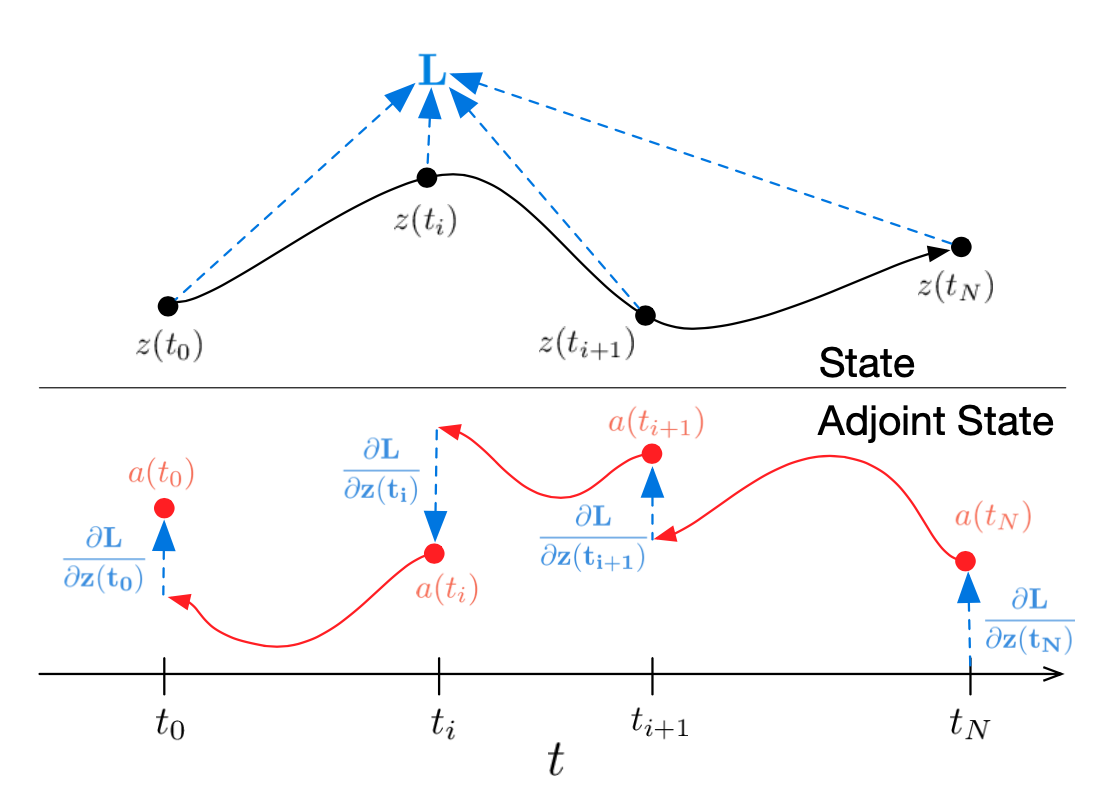
\includegraphics[width=0.75\linewidth]{adjoint_state.png}
        \caption{From \cite{chen2019neural}}
        \label{fig:adj_soln}
    \end{figure}

    % This figure tries to show dependence of loss on intermediate states, where reverse mode derivative is solved between each consecutive pair of output times
\end{frame}

\begin{frame}{Pseudocode}
    Solve reversed augmented ODE system, return the initial state and gradients (some mismatch in formulation and notation because of different solution choices for each of the adjoint steps, can double check!)
    \begin{figure}
        \centering
        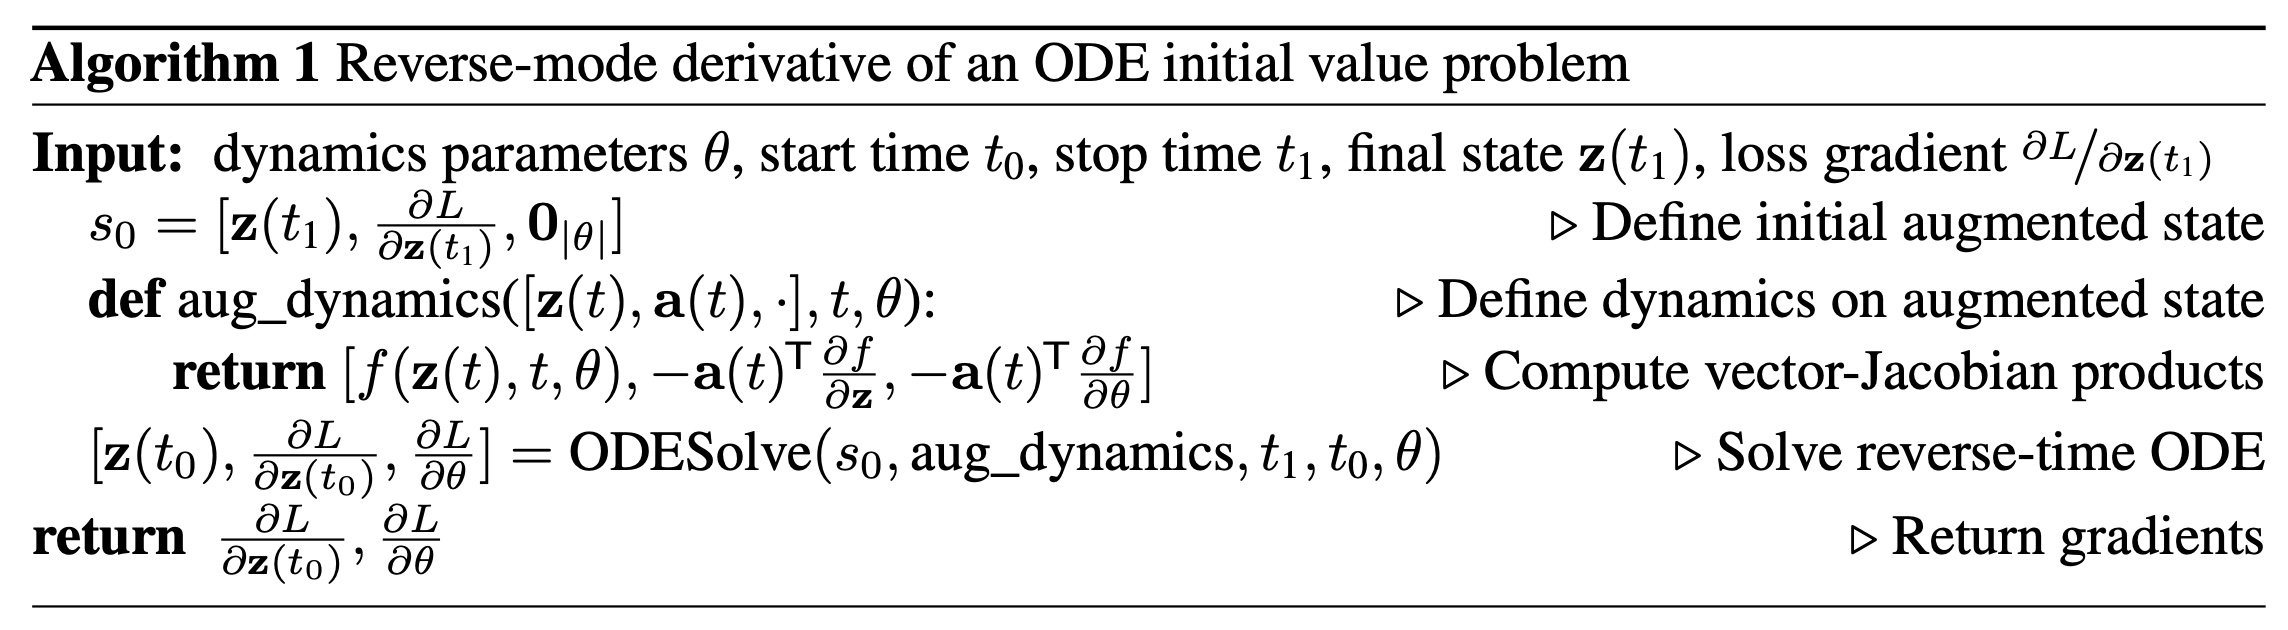
\includegraphics[width=\linewidth]{alg_revmode.jpg}
        \caption{From \cite{chen2019neural}}
        \label{fig:adj_alg}
    \end{figure}

\end{frame}


\begin{frame}{General Case (Prior Structural Information)}
    NODEs are a 1D Universal Differential Equation that is fully described by a neural network. \url{https://arxiv.org/pdf/2001.04385.pdf}

    $\mathcal{N}[u(t),u(\alpha(t)),W(t),U_\theta(u,\beta(t))]=0$

    where $W(t)$ is the Wiener process and $\alpha(t)$ is a delay function.

    Example 1: 
    Unknown stochastic features of $u$: $du=f(u,t)dt+g(u,U_\theta(u))dW_t$

    More general cases too! See TorchSDE \url{https://github.com/google-research/torchsde} for differentiable SDE solvers

    Example 2: Fisher-KPP 

    $\frac{\partial\rho}{\partial t}=r\rho(1-\rho)+D\frac{\partial^2\rho}{\partial x^2} \implies \rho_t=\mathrm{U}_\theta(\rho)+\hat{D}\operatorname{CNN}(\rho)$
    
\end{frame}

\begin{frame}{Related}
    \begin{itemize}
        \item We may need to solve for challenging BVPs too!
        
        \item BVPs as use case:
        \begin{itemize}
            \item SiREN: \url{https://www.vincentsitzmann.com/siren/}
            Periodic Activation functions to capture high-frequency information

            \item MOL-T (Method-of-Lines Transposed) \url{https://www.ams.org/journals/mcom/2014-83-290/S0025-5718-2014-02834-2/}

            \item Differentiable Multiple Shooting Layers \href{www.arxiv.org/abs/2106.03885}{Massaroli et al. 2021}
            
            Shooting: If BVP is $y''(t) = f(t, y(t), y'(t)), y(t_0)= y_0, y(t_1) = y_1$, solve IVP with $y'(t_0)=k$ s.t. $y(t_1, k) = y_1 \implies $ root finding.
        \end{itemize}
    \end{itemize}

    Competing Approach: Flow map learning (Churchill and Xiu 2023, \url{https://arxiv.org/pdf/2307.11013.pdf})
    
\end{frame}



% \begin{frame}{Applications of ODEs}
%     \url{https://tex.stackexchange.com/questions/693460/2-by-2-grid-of-subfigures-on-beamer-latex}
%     \begin{enumerate}
%         \item Building blocks in classification problems (last linear layer)

%         \item Dynamics of the latent state in encoder-decoder architecture

%         \item Point process models

%         \item Continuous normalizing flows

%         \item Probability flow ODEs in Diffusion Models?
%     \end{enumerate}

%     Notion of time is artificial in 1 and 4
% \end{frame}

\begin{frame}{Applications}
\begin{figure}    
    \begin{subfigure}[t]{.45\textwidth}
        \centering
        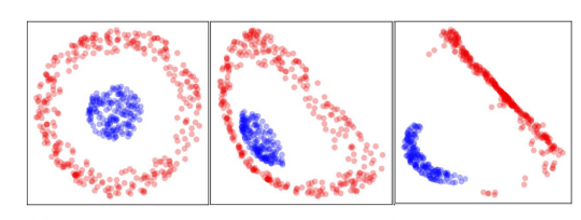
\includegraphics[width=.85\linewidth]{2d_class_node.png}
        \caption{Building block in e.g. classification \cite{dupont_augmented_2019}}
      \end{subfigure}
      \qquad
      \begin{subfigure}[t]{.45\textwidth}
        \centering
        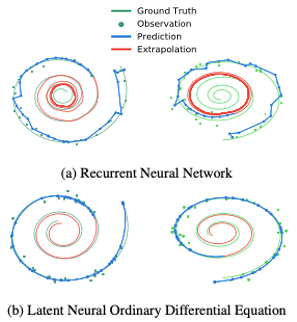
\includegraphics[width=.5\linewidth]{chen_latent_node.png}
        \caption{Encoder-Decoder latent state \cite{chen2019neural}}
      \end{subfigure}
    
      \medskip
    
      \begin{subfigure}[t]{.45\textwidth}
        \centering
        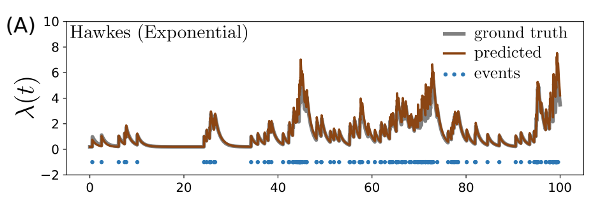
\includegraphics[width=.75\linewidth]{jia_hawkes.png}
        \caption{Temporal Point Process Model \cite{jia_neural_2020}}
      \end{subfigure}
      \qquad
      \begin{subfigure}[t]{.45\textwidth}
        \centering
        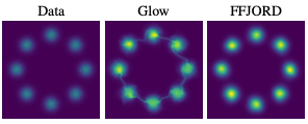
\includegraphics[width=.7\linewidth]{chen_cnf_2.png}
        \caption{Continuous Normalizing Flows (CNFs) \cite{grathwohl_ffjord:_2018}}
      \end{subfigure}
    \end{figure}
\end{frame}


\section{Dissecting Neural ODEs}

\begin{frame}{NFE}

    Section title comes from the nice paper by \cite{massaroli_dissecting_2021}

    \begin{enumerate}
        \item $f$ is integrated between $t_0$ and $t_k$, with a number of adaptive steps in between.

        \item The number of calls made to $f$ in the forward and backward pass are stored as NFE (number of function evaluations)

        \item Strategies that try to speed up training usually measure success by reduction in NFE.
    \end{enumerate}
\end{frame}

\begin{frame}{Adaptive ODE Solvers}
    % Notation borrowed from \cite{kidger_hey_2021}
    % High level steps: 
    $$y(t)=y(\tau)+\int_\tau^tf(s,y(s))\mathrm{~d}s$$

    Compute $\widehat{y}(t)$, step by $\Delta$ and generate $\widehat{y}_{\textrm{candidate}}(t + \Delta)$

    Estimate of solution size: $SCALE=ATOL+RTOL\cdot\max(\widehat{y}(t),\widehat{y}_\text{candidate}(t+\Delta))\in\mathbb{R}^d$

    \textbf{Error Ratio:} $r=\left\|\frac{y_{\mathrm{err}}}{SCALE}\right\|\in\mathbb{R}$, $r > 1 \implies$ reject, repeat smaller $\Delta$.

    \begin{figure}
        \centering
        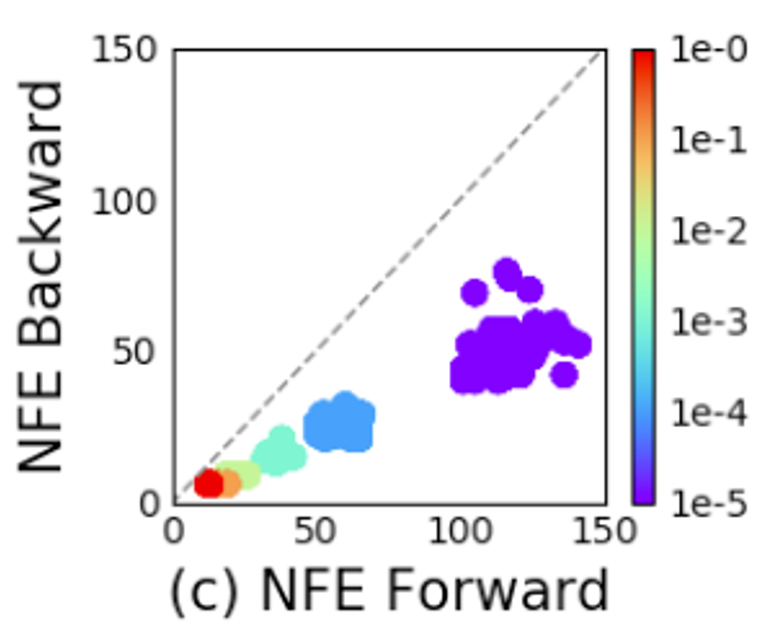
\includegraphics[width=0.32\linewidth]{NFE_Forward_vs_Backward.png}
        % \caption{Sample Test Trajectories from PNODE for CME Data}
        \label{fig:nfe}
    \end{figure}


    % However, this can be very stringent, too many small steps in backprop. 

    % Control dominant source of error in adjoint formulation i.e. $a_\theta$ and $a_t$ in $[a(t) a_{\theta}(t) a_t(t)]$ can be set to 0 at $\tau=T$. 
\end{frame}

\begin{frame}{Speed-up via seminorms}
    \begin{itemize}
        \item In practice this is very stringent, too many small steps taken in the reverse solve.
        
        \item Speeding up adjoint state calculation - \cite{kidger_hey_2021}
         
    \end{itemize}
\end{frame}

\begin{frame}{Speed-up via seminorms}
    Solve the following as a joint system.
    $$\begin{aligned}
        a_{\boldsymbol{z}}(T)& =\frac{\mathrm{d}L}{\mathrm{d}z(T)},  \\
        a_{\boldsymbol{\theta}}(T)& =0,  \\
        a_{\boldsymbol{t}}(T)& =\frac{\mathrm{d}L}{\mathrm{d}T},  \\
        a_{\boldsymbol{z}}(t)& =a_z(T)-\int_T^ta_z(s)\cdot\frac{\partial f}{\partial z}(s,z(s),\theta)\operatorname{d}s  \\
        \textcolor{red}{a_{\boldsymbol{\theta}}(t)}& \textcolor{red}{=a_\theta(T)-\int_T^ta_z(s)\cdot\frac{\partial f}{\partial\theta}(s,z(s),\theta)\operatorname{d}s}  \\
        \textcolor{red}{a_{\boldsymbol{t}}(t)}& \textcolor{red}{=a_t(T)-\int_T^ta_z(s)\cdot\frac{\partial f}{\partial s}(s,z(s),\theta)\operatorname{d}s}
    \end{aligned}$$

    $z$ for $a_{\boldsymbol{z}}$ is (typically) recovered by solving original ODE backwards-in-time.

\end{frame}

\begin{frame}{Hey that's not an ODE!}
    In fact, $a_{\boldsymbol{\theta}}(t)$ and $a_{\boldsymbol{t}}(t)$ are merely integrals and not ODEs (dependence on $a_{\boldsymbol{z}}$ instead of original adjoint variable).

    $\implies$ \textcolor{red}{Only stringent requirements are for $z$ and $a_{\boldsymbol{z}}$ (ensuring small errors do not propagate)}

    Proposed method: Check error ratio only for $z$ and $a_{\boldsymbol{z}}$, zero weight for the remaining augmented states to avoid spurious rejections!

    Their results: NFE Backward $\downarrow$ by median 40\%, NFE Total $\downarrow$ by as much as 62\%.
\end{frame}


% \begin{frame}{Seminorms}

% \end{frame}

\begin{frame}{Choice of augmentation / data control}
    ODE trajectories for different ICs will not intersect i.e. if $h_1(0) \neq h_2(0)$, $h_1(t) \neq h_2(t)$ - \emph{NODEs must preserve the topology of the input space} \href{https://physics.stackexchange.com/questions/578836/paths-in-phase-space-can-never-intersect-but-why-cant-they-merge}{also see Intersection of Paths in Phase Space}

    But with discrete data (e.g. concentric annuli), the model will stretch a part of 2D space and eventually separate classes $\implies$ more complex flow, $\uparrow$NFEs.

    \textbf{Trick:} Lift from $\mathbb{R}^d$ to $\mathbb{R}^{d + p}$: 
    
    $$\frac{\mathrm d}{\mathrm dt}\begin{bmatrix}\mathbf h(t)\\\mathbf a(t)\end{bmatrix}=\mathbf f\left(\begin{bmatrix}\mathbf h(t)\\\mathbf a(t)\end{bmatrix}, t\right),\quad\begin{bmatrix}\mathbf h(0)\\\mathbf a(0)\end{bmatrix}=\begin{bmatrix}\mathbf x\\\mathbf0\end{bmatrix}$$

    (see \cite{dupont_augmented_2019}) 
    
    Implement and visualize: \href{https://uvadlc-notebooks.readthedocs.io/en/latest/tutorial_notebooks/DL2/Dynamical_systems/dynamical_systems_neural_odes.html}{UVA DL Tutorials} (switch to ppt)

    % 1D trajectories won't intersect, 2D can though? (for individual dimensions that is.)
\end{frame}

\begin{frame}{Second Order NODEs}
    (see \cite{Norcliffe2020} for more formal interpretation)
    % Unlike the original ANODE
    % , they allow $\mathbf{a}(0)$ to be learnt as a function of $\mathbf{h}(0)$ by a neural network $g$.

    $\frac{\mathrm d}{\mathrm dt}\begin{bmatrix}\mathbf h(t)\\\mathbf a(t)\end{bmatrix}=\mathbf f\left(\begin{bmatrix}\mathbf h(t)\\\mathbf a(t)\end{bmatrix}, t\right),\quad\begin{bmatrix}\mathbf h(0)\\\mathbf a(0)\end{bmatrix}=\begin{bmatrix}\mathbf x\\\textcolor{red}{g(\mathbf{h}(0), \theta_g)}\end{bmatrix}$

    Second order system  - solve for $y$ using augmentation with $a$:
    $\mathbf{y}(t_0)=\mathbf{y}_0,\quad\quad\dot{\mathbf{y}}(t_0)=g(\mathbf{y}(t_0),\theta_g),\quad\quad\ddot{\mathbf{y}}=f^{(a)}(\mathbf{y},\dot{\mathbf{y}},t,\theta_f)$

    % which can be interpreted as:
    $\mathbf{z}=\begin{bmatrix}\mathbf{y}\\\mathbf{a}\end{bmatrix},\, \dot{\mathbf{z}}=f^{(v)}(\mathbf{z},t,\theta_f)=\begin{bmatrix}\mathbf{a}\\f^{(a)}(\mathbf{y},\mathbf{a},t,\theta_f)\end{bmatrix},\,\mathbf{z}(t_0)=\begin{bmatrix}\mathbf{y}_0\\g(\mathbf{y}_0,\theta_g)\end{bmatrix}$

    \textcolor{blue}{\emph{For tasks such as classification (where trajectory is unimportant), ANODEs can access higher order dynamics and might perform better compared to second order formulation.}}

\end{frame}

% \begin{frame}{Example: Binary Classification}
%     \includemedia[
%         activate=pageopen,
%         width=200pt,height=150pt,
%         addresource=2d_classification.mp4, % Specify the path to your video file here
%         flashvars={
%          source=2d_classification.mp4  % Same video file path as above 
%          &autoPlay=true,        % Change to false to prevent autoplay
%          &loop=false             % Change to false to prevent loop
%         }
%       ]{}{VPlayer.swf}
% \end{frame}

% \begin{frame}{Choice of Dimensionality}

% \end{frame}

\begin{frame}{Choice of Regularization}
    % Path dependence (thermodynamics) \url{https://iopscience.iop.org/article/10.3847/1538-4365/ab340c}
    Reference: \cite{finlay_how_2020}

    \begin{figure}
        \centering
        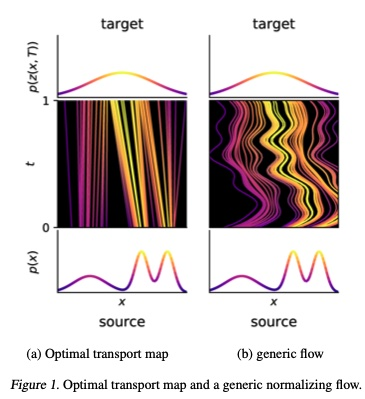
\includegraphics[width=0.6\linewidth]{ot_vs_generic_NF.jpg}
        \caption{Regularized flow for NF}
        \label{fig:reg_ot}
    \end{figure}
\end{frame}

\begin{frame}{Choice of Regularization}
    $$\begin{cases}\dot{\mathbf{z}}=\mathbf{f}(\mathbf{z},t;\theta)\\\mathbf{z}(0)=\mathbf{x}\end{cases}$$

  (\emph{If well-conditioned, we should exert nearly constant force on particles}). Regularize terms from total derivative for $f$! 

    $$\begin{aligned}
        {\frac{\mathrm{d}\mathbf{f}(\mathbf{z},t)}{\mathrm{d}t}}& =\nabla\mathbf{f}(\mathbf{z},t)\cdot\dot{\mathbf{z}}+\frac{\partial\mathbf{f}(\mathbf{z},t)}{\partial t}  \\
        &=\textcolor{red}{\nabla\mathbf{f}(\mathbf{z},t)}\cdot\textcolor{blue}{\mathbf{f}(\mathbf{z},t)}+{\frac{\partial\mathbf{f}(\mathbf{z},t)}{\partial t}}
        \end{aligned}$$

    Introduce regularization terms which can be solved as an augmented ODE.\footnote{There are other ways to promote easy-to-integrate dynamics too, e.g. by regularizing higher-order derivatives of $f$, see section 5.4 of \cite{kidger_neural_2022}.}
\end{frame}

\begin{frame}{Choice of Regularization}
    Quadratic cost transport map between $p(\mathbf{x})$ and $q(\mathbf{x})$:

    $$\begin{aligned}M(\mathbf{z})=\int\|\mathbf{x}-\mathbf{z}(\mathbf{x})\|^2p(\mathbf{x})\mathrm{d}\mathbf{x}\end{aligned}$$

    s.t. $\int_Aq(\mathbf{z})\mathrm{d}\mathbf{z}\int_{\mathbf{z}^{-1}(A)}p(\mathbf{x})\mathrm{d}\mathbf{x}$

    Minimize measure of kinetic energy of flow (presenting results as is for now):
    $$\begin{aligned}
        &\textcolor{red}{\min_{f,\,\rho}}&& \textcolor{red}{\int_0^T\int\|\mathbf{f}(\mathbf{x},t)\|^2\rho_t(\mathbf{x})\mathrm{d}\mathbf{x}\mathrm{d}t}  \\
        &\text{subject to}&& \begin{aligned}\frac{\partial\rho_t}{\partial t}&=-\operatorname{div}\left(\rho_t\mathbf{f}\right),\end{aligned}  \\
        &&&\rho_0(\mathbf{x})=p, \\
        &&&\rho_T(\mathbf{z})=q.
    \end{aligned}$$
\end{frame}

\begin{frame}{Choice of Regularization}
Pseudocode:

\begin{figure}
    \centering
    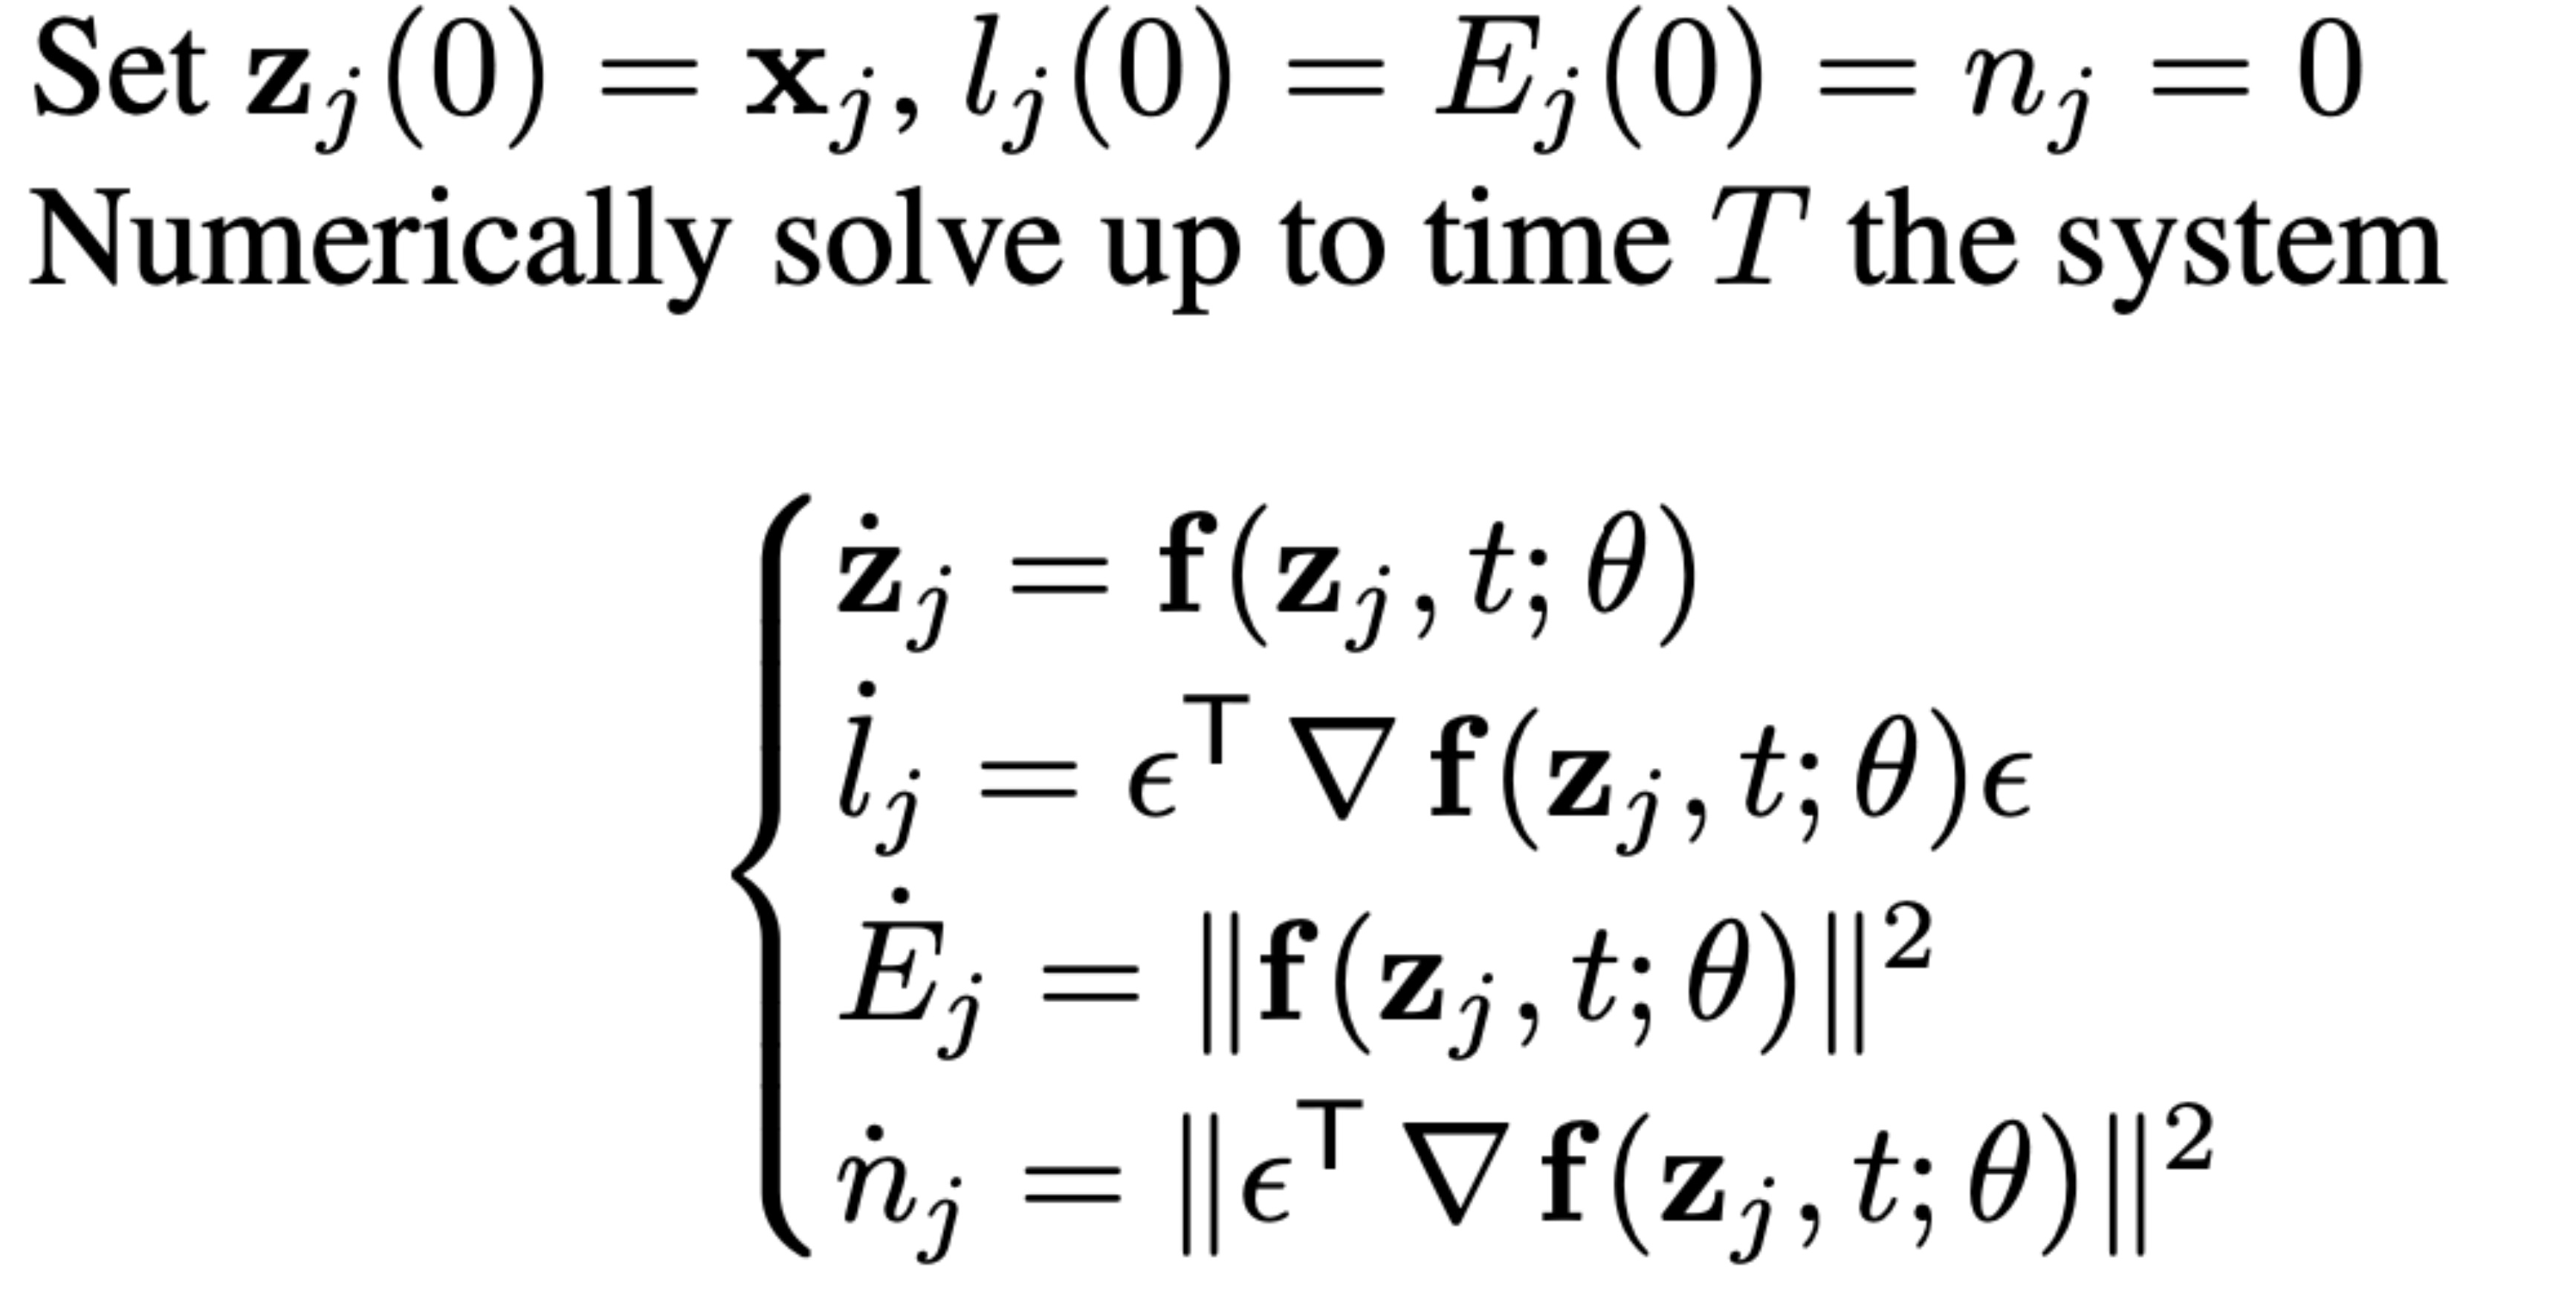
\includegraphics[width=0.5\linewidth]{finlay_rnode.jpg}
    \caption{Augmented system solved for RNODE from \cite{finlay_how_2020}}
    \label{fig:reg_finlay}
\end{figure}


\end{frame}

\begin{frame}{Event Function Handling}
    Termination of \texttt{ODESolve} is handled implicitly by the event function (useful for switching dynamics, collisions, temporal point processes)

    \begin{figure}
        \centering
        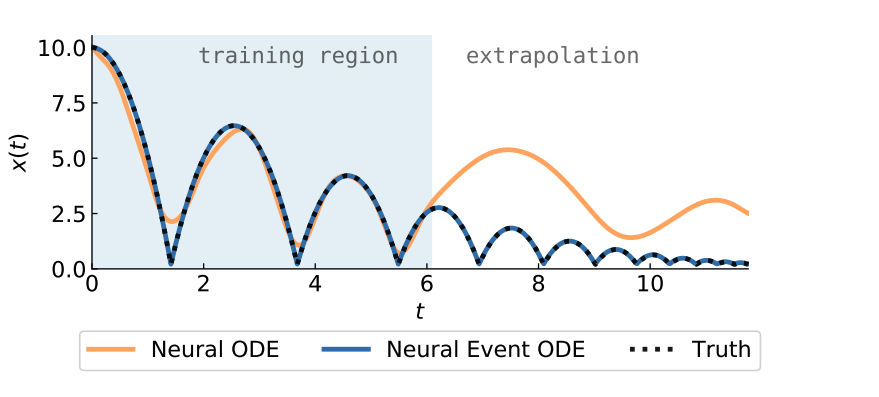
\includegraphics[width=0.5\linewidth]{bouncing_ball.png}
        \caption{From Kidger et al. \url{https://arxiv.org/pdf/2011.03902.pdf}. Solve $t^{\ast}, z(t^{\ast}) = \textrm{ODESolve}(z_0, f, g, t_0)$ where $g = x(t) - r$}
        \label{fig:bball_neural_event_function}
    \end{figure}
\end{frame}

% \begin{frame}{Parametrization}
    
% \end{frame}

\begin{frame}{Parametrized Neural ODEs}
    \begin{columns}
        \begin{column}{0.51\textwidth}
            \begin{figure}
                \centering
                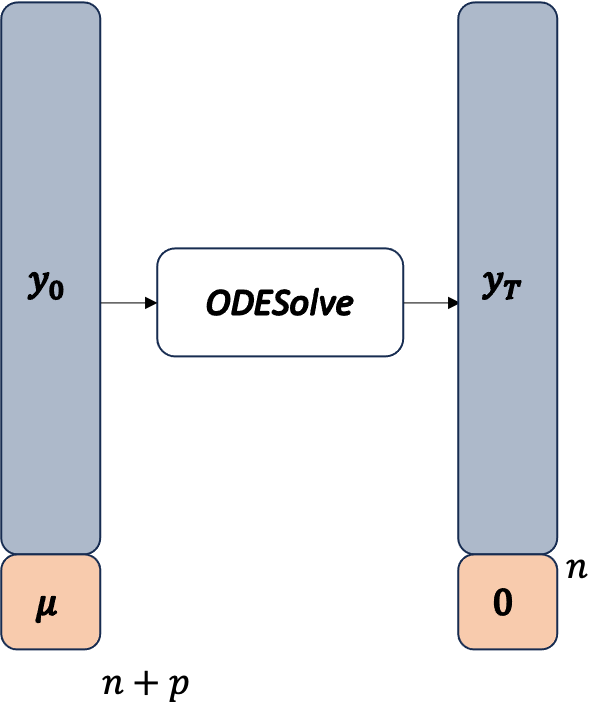
\includegraphics[width=0.7\linewidth]{pnode_idea.png}
                % \caption{Enter Caption}
                \label{fig:pnode_idea}
            \end{figure}
        \end{column}
        \begin{column}{0.52\textwidth}
            \begin{itemize}
                \item  Reminiscent of e.g. Conditional VAEs - guided generation of samples based on label information from the decoder, e.g. pNNs in HEP Applications \cite{anzalone_improving_2022}
                
                \item Similar to \cite{lee_parameterized_2021}, but they have an additional encoder-decoder setup i.e. NODEs are solved in latent space.
    
                \item Some connections to `Partially Input Convex Neural Networks' \cite{amos_input_2017}
    
                % \item Conditional OT Estimation, or Neural Optimal Transport With Context, PICNN (Partially Input Convex Neural Networks) - see Chapter 5 of \cite{bunne_neural_2023} and perhaps \cite{amos_input_2017} - possible applications being structured prediction, data imputation and inference?
            \end{itemize}
        \end{column}
    \end{columns}
\end{frame}

\begin{frame}{Summing up...}
\textbf{Advantages:}

\begin{enumerate}
\item Memory savings - with various tricks can avoid storing intermediate activations to get gradients of loss function.
% as knowing the state at any $t$ we can reconstruct the trajectory forwards and backwards - see algebraic and analytic reversibility in Kidger et al. 2022! (section 5.3.2.1)
(basic selling point of implicit layer based methods!)

\item Tractable normalizing flows without restrictive architectures by replacing the $|\cdot|$ with a trace approximation (see FFJORD \cite{grathwohl_ffjord:_2018}) (haven't reproduced any detailed experiments for speedups, log-likelihood vs common NF architectures)

\item Fairly simple implementation of a NODE layer in existing DL frameworks with plugin of standardized ODE solvers 

\item More general framework of UDEs permits us to mix in prior knowledge of some terms and extend to more systematic discovery with sparse regression
\end{enumerate}
\end{frame}

% \begin{frame}{Summing up...}
% \textbf{Drawbacks}
% \begin{enumerate}

% \item Choice of activations (tanh, ReLU etc.) can throw up poor results, very problem-dependent. Lack of restriction on architecture is not necessarily a blessing. (see \cite{sitzmann_implicit_2020}).

% \item Gradients through continuous adjoints carry numerical error (error in terminal condition from forward pass, solution of adjoint states)

% \end{enumerate}
% \end{frame}

\begin{frame}{Summing up}
    \textbf{Drawback:}
    Can struggle to handle more than a few tens of state dimensions, image data (big fully connected layers).

    \begin{itemize}
        \item \cite{lee_parameterized_2021} solve NODEs in 5-7 dimensional latent space which is really fast.
        
        \item Flow Maps - \textcolor{blue}{``No matter
        what approximation method is used inside the interval [TL, TU ], numerical accuracy
        can not be ensured outside the interval [TL, TU ], especially far beyond it. ''}
        \textcolor{blue}{``Therefore, if
        a temporal approximation $\tilde{x}(t)$ is sought after in a learning method, the method will not provide accurate predictions beyond the training time domain [TL, TU ]''}
    \end{itemize}
\end{frame}

\section{Experiments and Rough Results}
% \section{Conformal Prediction}
% \begin{frame}{EnBPI for Time Series}
%     Reference: \cite{xu_conformal_2023}
% \end{frame}
% \begin{frame}{Definition}
%     \cite{amos_input_2017}
% \end{frame}

% \begin{frame}{Inductive CP}
% \end{frame}

% \begin{frame}{Coverage Properties}
    
% \end{frame}

\begin{frame}{Application}
    White Light Images with Overlaid Edges: \url{https://drive.google.com/file/d/1KSiu1n7Q0TC4Zy_F_3QU0rSFrM-KBNLt/view?usp=sharing}

    \textbf{Abuse of notation:} Initial condition $t_0$ is treated as state values for first appearance in coronagraph $\implies$ we still have to run fresh simulations to generate these ICs in the first place.

    \textbf{Utility: } Good for rough approximation of kinematics as far as correlation with arrival time is concerned, but lot of details (3 part structure etc.) lost by dropping the images.

    % \textbf{Possible extension: } Domain adaptation - Transfer pretrained model to new CME event with only a few tens of simulations available.
    
\end{frame}

\begin{frame}{Batch for training PNODEs}
    Two step sampling - sample $n$ simulations at different $\mu$ followed by $m$ ICs from different $t_i$, integrate each IC from each time series up to $k$ timesteps - $n \times m \times k \times (d + p)$ tensor.

\begin{table}[]
\centering
\begin{tabular}{cllll}
                          & $i_1$                    & $i_2$                    & $\cdots$ & $i_m$                    \\
\multirow{3}{*}{$j_1$}        & $y_0^{(i_1)}(\mu_{j_1})$     & $y_0^{(i_2)}(\mu_1)$     &          & $y_0^{(i_m)}(\mu_{j_1})$     \\
                          & $\cdots$                 & $\cdots$                 &          & $\cdots$                 \\
                          & $y_{k-1}^{(i_1)}(\mu_{j_1})$ & $y_{k-1}^{(i_2)}(\mu_{j_1})$ &          & $y_{k-1}^{(i_m)}(\mu_{j_1})$ \\
\multirow{3}{*}{$\vdots$} &                          &                          &          &                          \\
                          &                          & $\vdots$                 &          &                          \\
                          &                          &                          &          &                          \\
\multirow{3}{*}{$j_n$}        & $y_0^{(i_1)}(\mu_{j_n})$     & $y_0^{(i_2)}(\mu_{j_n})$     &          & $y_0^{(i_m)}(\mu_{j_n})$     \\
                          & $\cdots$                 & $\cdots$                 &          & $\cdots$                 \\
                          & $y_{k-1}^{(i_1)}(\mu_{j_n})$ & $y_{k-1}^{(i_2)}(\mu_{j_n})$ &          & $y_{k-1}^{(i_m)}(\mu_{j_n})$
\end{tabular}
% \caption{}
\label{tab: train_tensor}
\end{table}
\end{frame}

% \begin{frame}{Sequential Predictive Conformal Inference}
%     Reference: \url{https://proceedings.mlr.press/v202/xu23r/xu23r.pdf} \cite{pmlr-v202-xu23r}
% \end{frame}

% \begin{frame}{Coverage Properties, Pinball Loss etc}
    
% \end{frame}

% \section{Results}

\begin{frame}{Synthetic Example}
    `Time series' defined by truncated cardioid curves with varying rate of change in $a$ i.e. 1 input parameter. $r(\theta) = a(1 + \cos (\theta))$

    2 time series to train, 1 as validation (interpolate), 1 as test (extrapolate)

    \begin{figure}
        \centering
        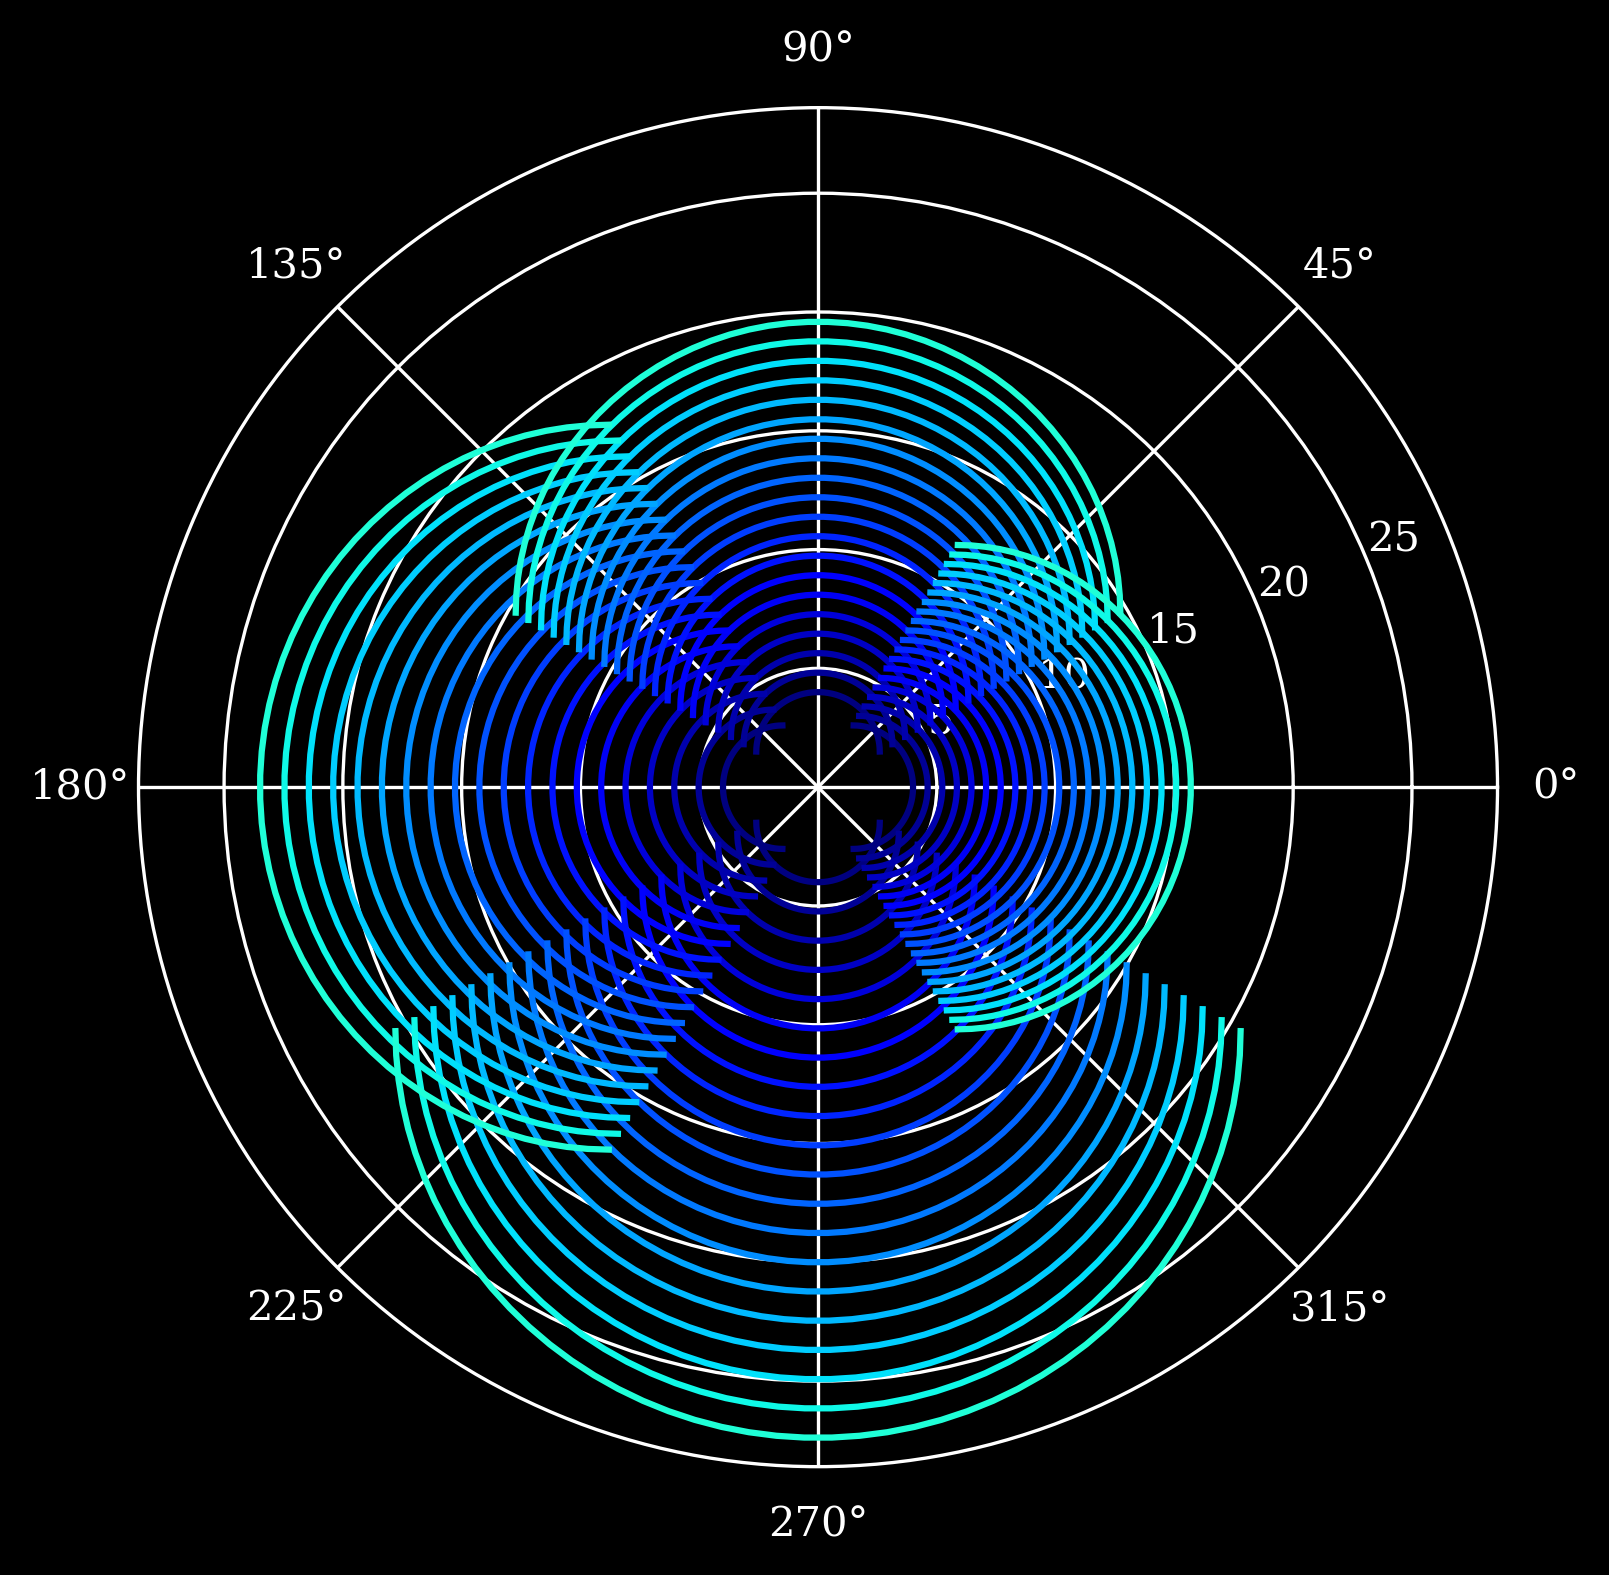
\includegraphics[width=0.4\linewidth]{cardioid_curves.png}
        % \caption{}
        \label{fig:cc1}
    \end{figure}

\end{frame}

\begin{frame}{Synthetic Example}
50-dimensional, 2 hidden layers, 2000 iterations.
Reproduces time-series on training simulations.
\begin{figure}
    \centering
    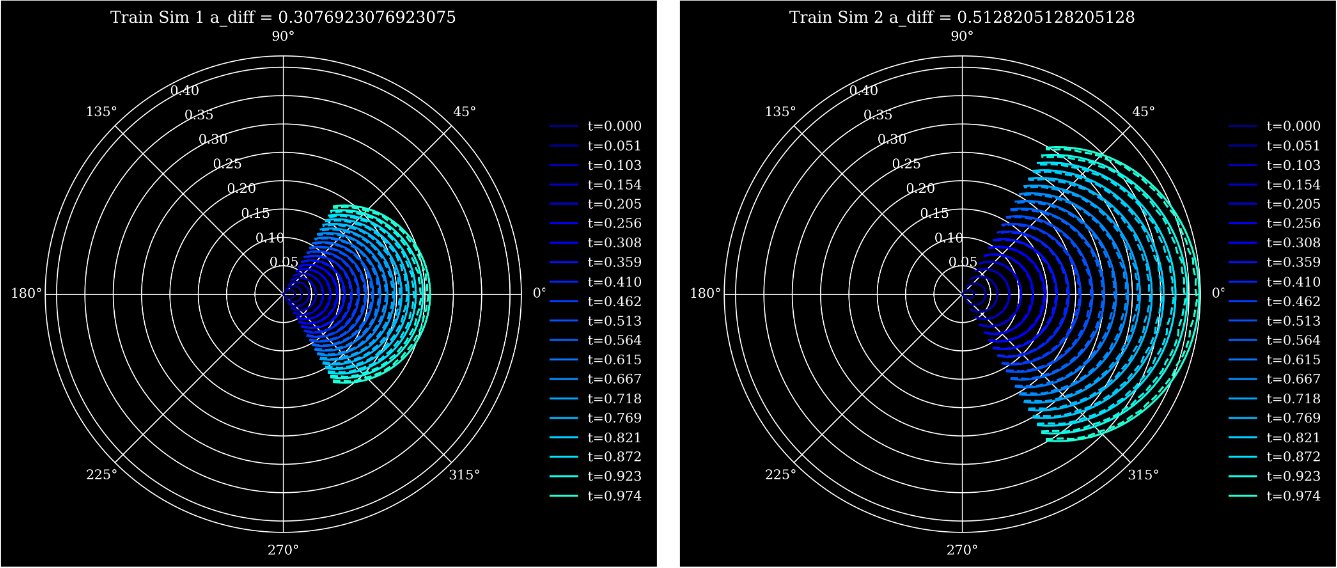
\includegraphics[width=\linewidth]{Training_reproduction.png}
    % \caption{}
    \label{fig:cc2}
\end{figure}
\end{frame}

\begin{frame}{Synthetic Example}
Validation and Test Results (only IC supplied for each) - struggles only in pure extrapolation.
\begin{figure}
    \centering
    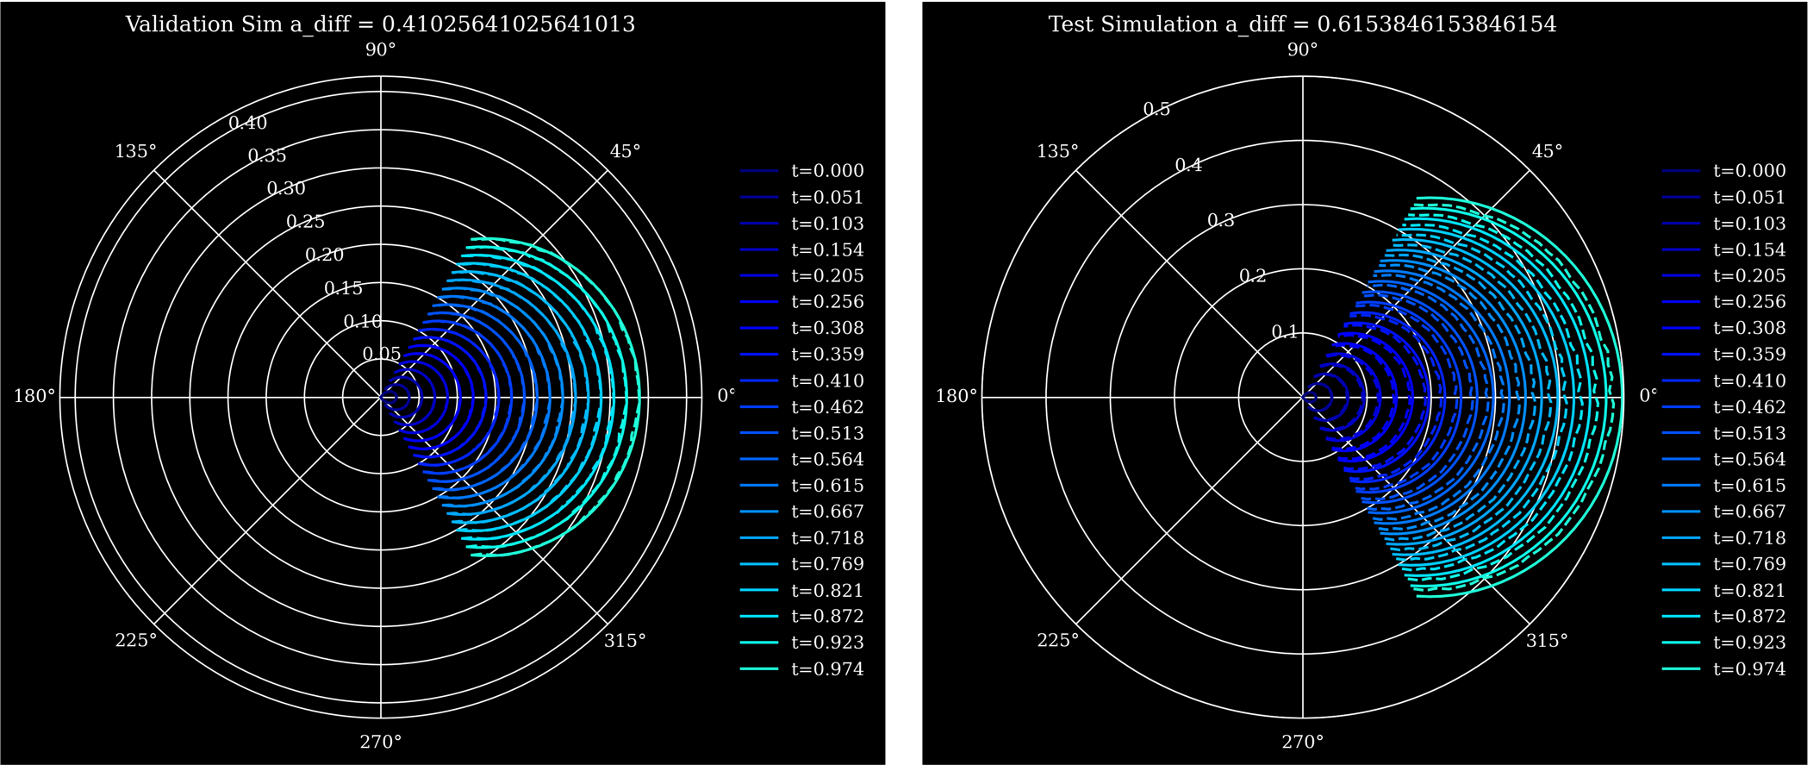
\includegraphics[width=\linewidth]{cardioid_curves3.png}
    % \caption{}
    \label{fig:cc3}
\end{figure}

\end{frame}

\begin{frame}{Actual Example :-(}
183 training trajectories, 40 test trajectories of CME leading edge propagation, 4 simulations per batch. 10-dimensional parameter space.

\begin{figure}
    \centering
    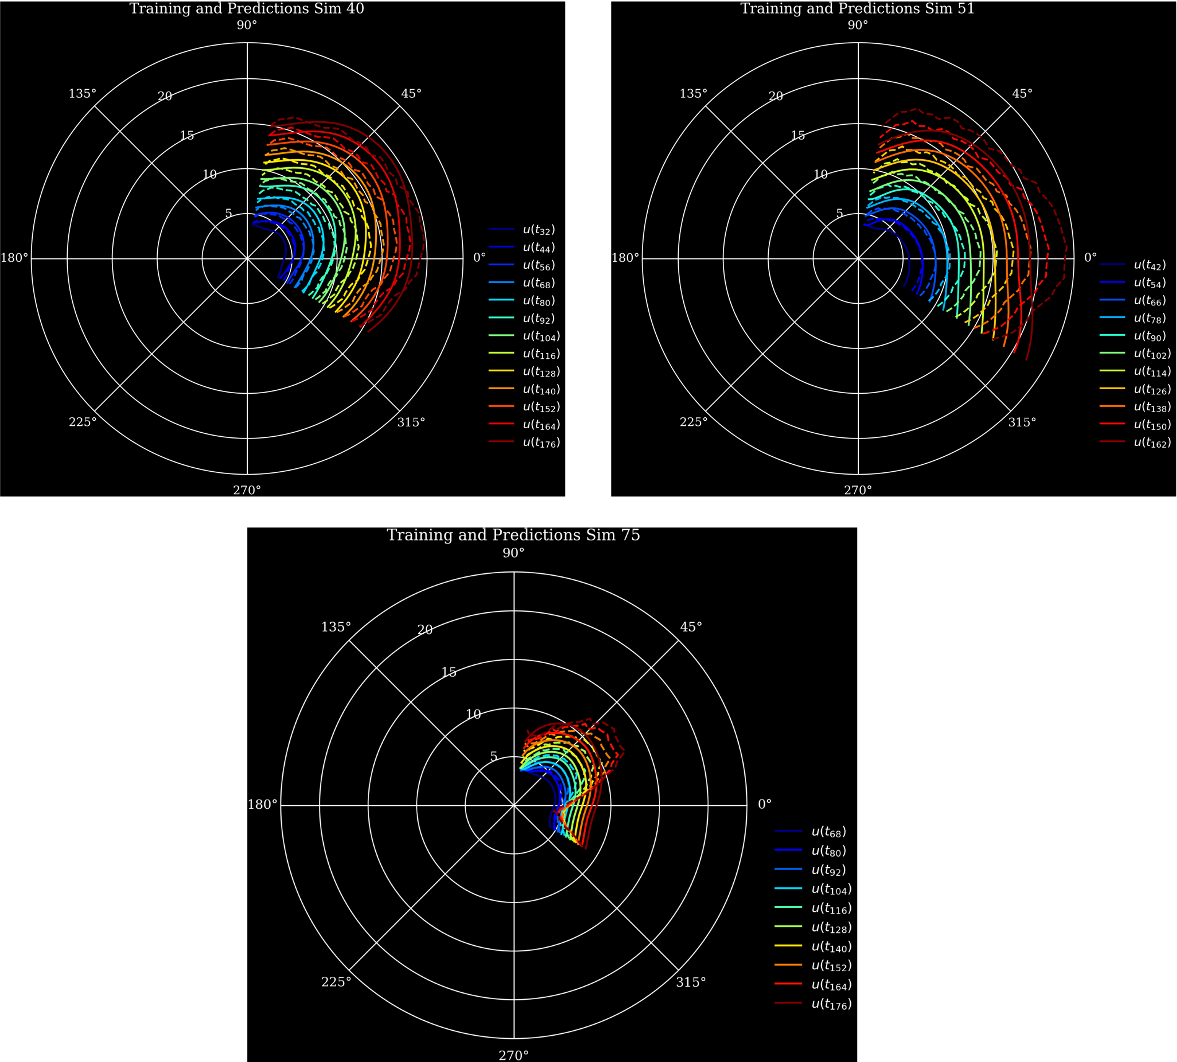
\includegraphics[width=0.6\linewidth]{CME_test_samples.png}
    % \caption{Sample Test Trajectories from PNODE for CME Data}
    \label{fig:cc4}
\end{figure}
\end{frame}

\begin{frame}{Conformal Prediction}
    \cite{shafer08} Given data $\mathcal{D}_{n - 1} = {(x_1, y_1), (x_2, y_2), \cdots (x_{n-1}, y_{n-1})}$, predict $y_n$ via some algorithm $\mathcal{A}$:

    $$\hat{y_n} = \mathcal{A}((x_1, y_1), (x_2, y_2), \cdots (x_{n-1}, y_{n-1}))$$

    \pause

    For some error probability $\alpha$, find prediction set such that:

    $$\mathrm{P}\left(y_{n}\in\Gamma^{\alpha}((x_{1}, y_1),(x_{2}, y_2),\ldots,(x_{n-1}, y_{n-1}), x_n)\right)\geq(1-\alpha)$$

    \textcolor{red}{Marginal coverage: Guarantee holds over all possible draws of $x_{n}$}

\end{frame}

\begin{frame}{Vanilla Split Conformal}

\begin{itemize}
\item Split $\mathcal{D}_{n-1}$ into disjoint $\mathcal{D}_{n-1}^{(1)}$ and $\mathcal{D}_{n-1}^{(2)}$ \textcolor{red}{ - calibration set}

\item Train model on $\mathcal{D}_{n-1}$

\item Evaluate non-conformity measure \footnote{should satisfy some intuition i.e. correctly rank inputs from highest to lowest magnitude of model error for sets to be useful.} (any suitable error or discrepancy) on $\mathcal{D}_{n-1}^{(2)}$ and test sample $\mathbf{x}^{\ast}$

\item $\alpha_i=\begin{cases}|y_i-\widehat{\mu}(\mathbf{x}_i)|,&1\le i\le|\mathcal{D}_{n-1}^{(2)}|\\|y-\widehat{\mu}(\mathbf{x}^{\ast})|,&\text{for testing sample}\end{cases}$

\item Resulting Prediction Set:
$\Gamma^{\alpha}((x_{1}, y_1),(x_{2}, y_2),\ldots,(x_{n-1}, y_{n-1}), \mathbf{x^{\ast}}) = [\widehat{\mu}(\mathbf{x}^*)-d,\widehat{\mu}(\mathbf{x}^*)+d]$

$d=$ the $\lceil(1-\alpha)(|\mathcal{D}_{n-1}^{(2)}|+1)\rceil$ smallest of $\alpha_{1},\ldots,\alpha_{|\mathcal{D}_{n-1}^{(2)}|}$
\end{itemize}
\end{frame}

\begin{frame}{Some initial results}
(for our case, $x_i$ is joint IC and parameter values i.e. $y_0^{(i)}, \mu^{(i)}$, prediction is $y_t^{(i)}$, prediction algorithm $\mathcal{A}$ is $\textrm{ODESolve}(y_0^{(i)}, \mu^{(i)}, t_0, t_i)$)

\pause

All predictions in time from the IC will have the same fixed intervals from this method, doesn't adapt to better or worse predictions.

\end{frame}

\begin{frame}{Some initial results}

    \begin{figure}
        \centering
        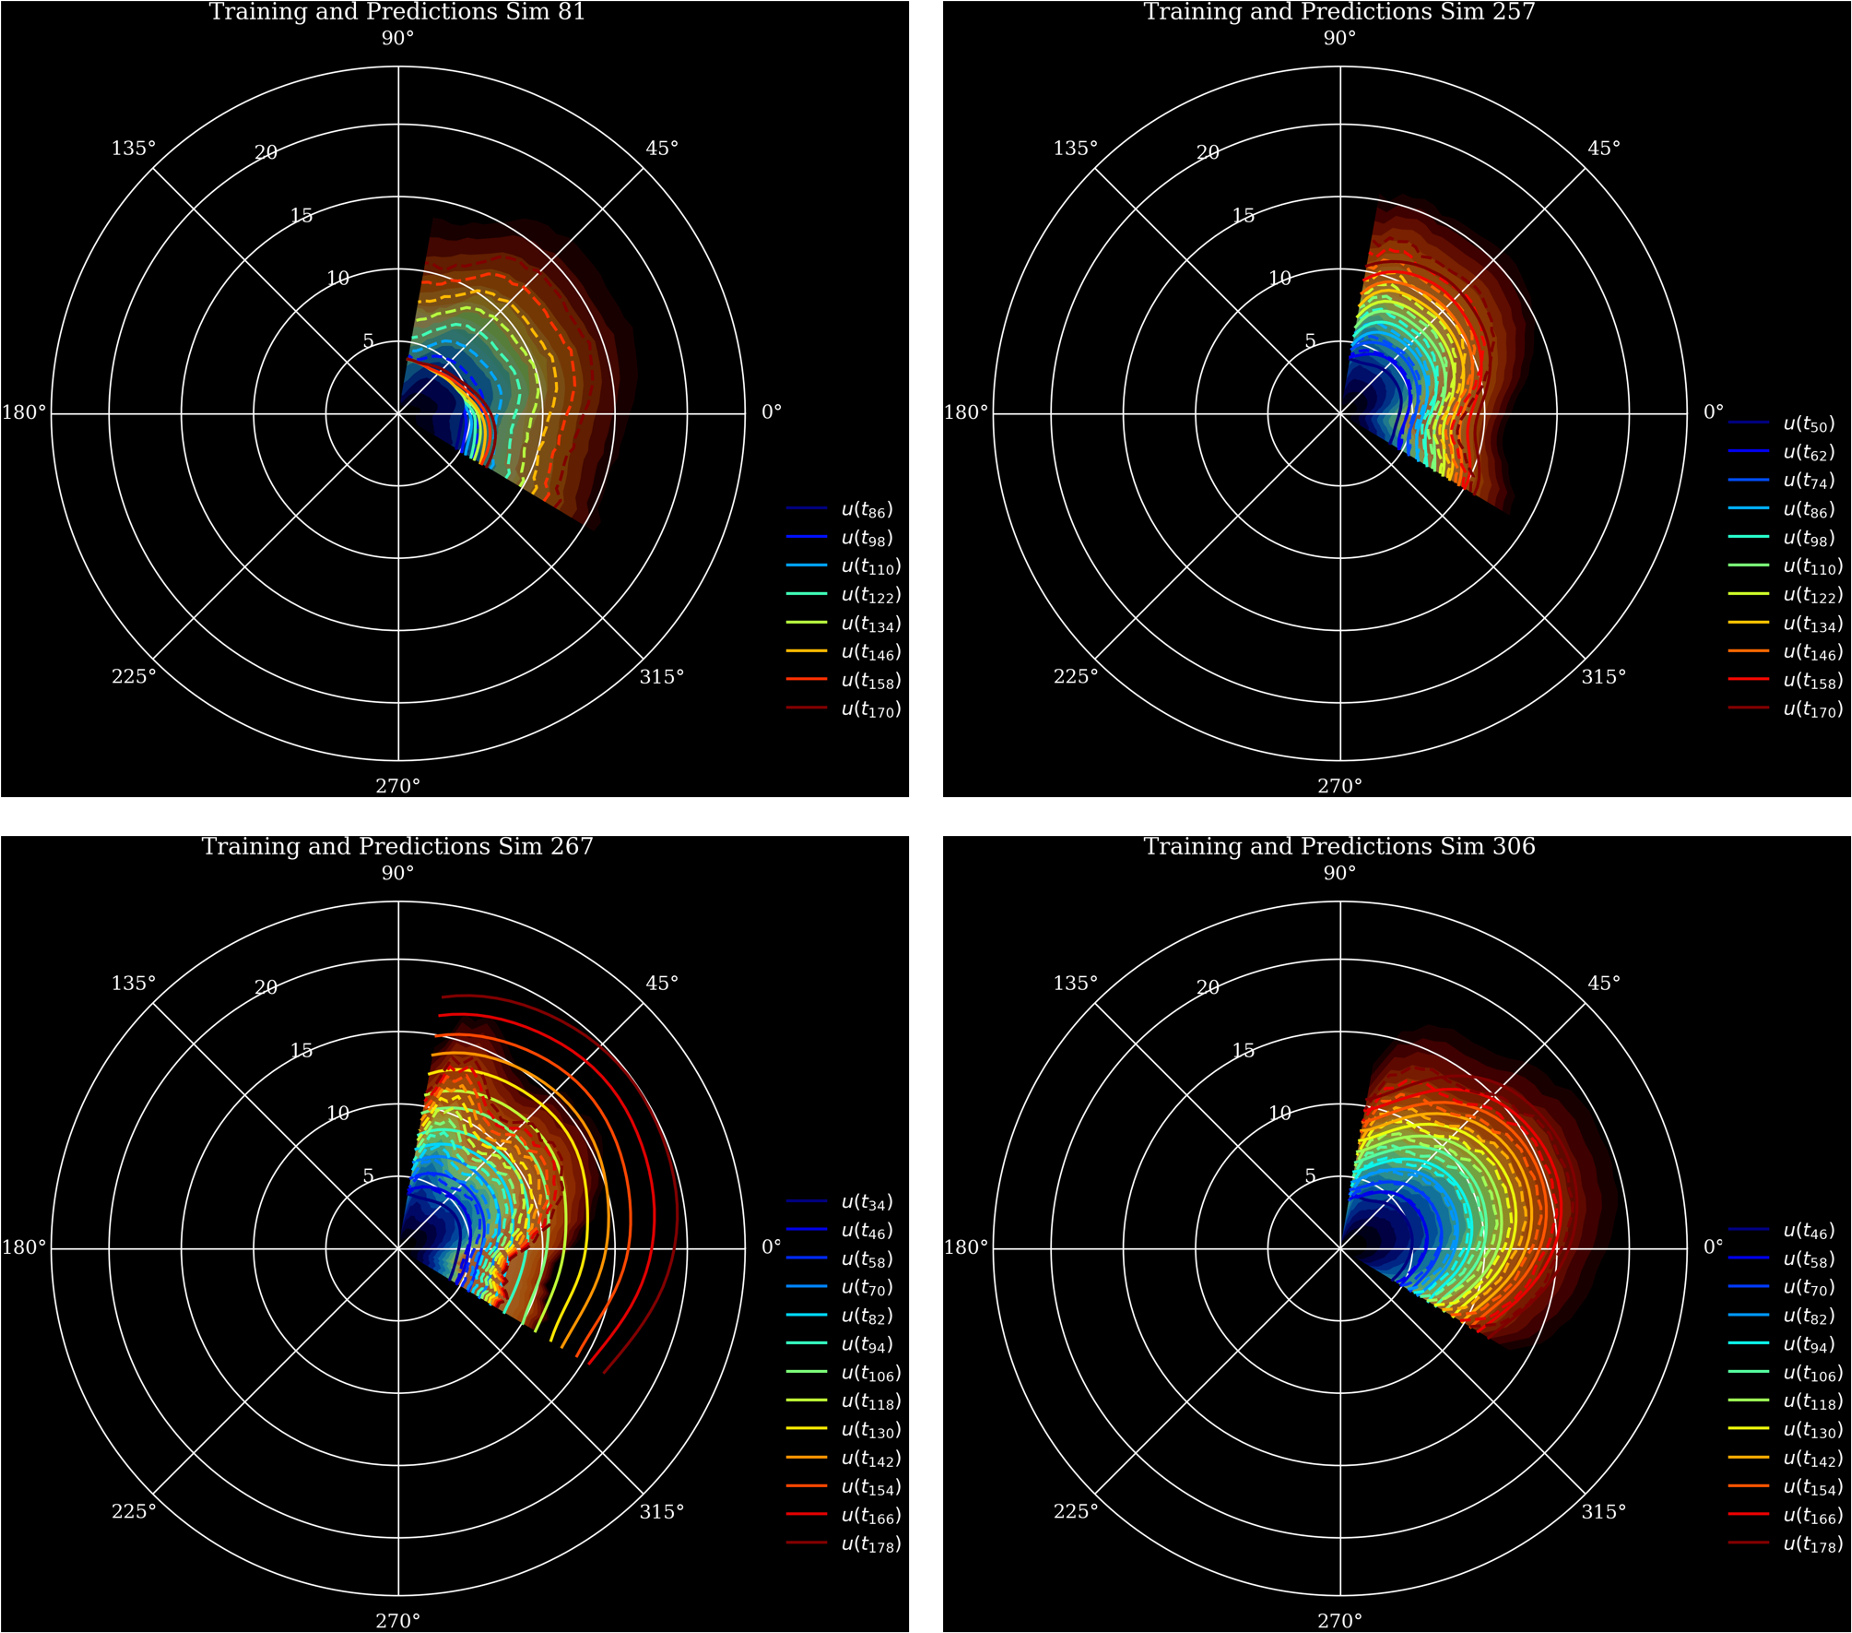
\includegraphics[width=0.8\linewidth]{intervals_fixedcp.png}
        % \caption{Figure from \cite{angelopoulos_gentle_2022}}
        \label{fig:cp_fixed_res}
    \end{figure}

\end{frame}



\begin{frame}{Major challenges}
\begin{enumerate}
    \item Improved interpolation capabilities of NODEs with high-dimensional $\mu$ (better embeddings, architectures?)

    \item ``Adaptive'' intervals - more efficient prediction sets that are smaller for test points where model is more accurate
    
    \textcolor{red}{This typically requires a prior method that does some of the heavy lifting on constructing intervals e.g. quantile regression, and CP essentially calibrates them to satisfy our guarantee}

    \item (Can't do much about this): For a given choice of calibration set size, how far off are we from the marginal guarantee of $1 - \alpha$? 

    % \item Handling covariate shifts (source to target event?)
\end{enumerate}
\end{frame}

\begin{frame}{Number of samples}
    Run calibration algorithm multiple time, sampling a new calibration set and check the coverage.

    \begin{figure}
        \centering
        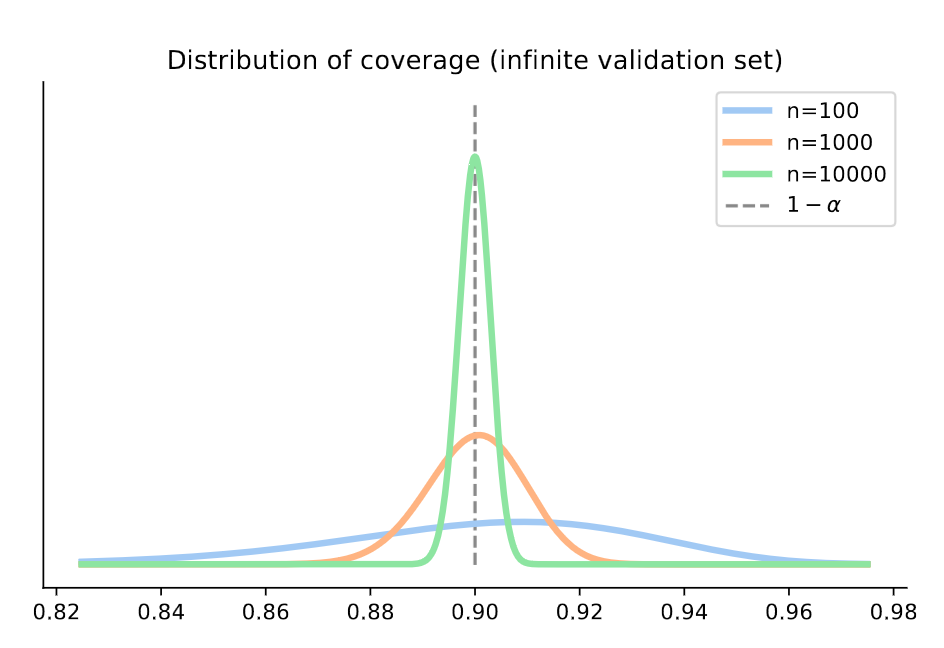
\includegraphics[width=0.5\linewidth]{coverage_distribution.png}
        \caption{Figure from \cite{angelopoulos_gentle_2022}}
        \label{fig:cdist}
    \end{figure}


    Typically need order of $10^3$ calibration samples to ensure we are within a given $\epsilon=0.2$.
\end{frame}


\begin{frame}{Slightly modified score function}
    \cite{angelopoulos_gentle_2022} Come up with a heuristic notion for $\sigma$ i.e. define $u(x)$ such that larger values encode more uncertainty. \footnote{drawback?: no reason to believe that estimate of $\sigma$ is directly related to quantiles of label distribution - usually best coverage comes from quantile regression if feasible.}
    
    e.g. measure variance of $\widehat{\mu}(x)$ to random input perturbations, get so-called `standardized' scores $\alpha_i = \frac{|y_i - \widehat{\mu}(\mathbf{x}_i)|}{u(\mathbf{x}_i)}$
    
    Then: 
    $\Gamma^{\alpha}((x_{1}, y_1),(x_{2}, y_2),\ldots,(x_{n-1}, y_{n-1}), \mathbf{x^{\ast}}) = [\widehat{\mu}(\mathbf{x}^*)-d,\widehat{\mu}(\mathbf{x}^*)+d]$

    where $d=u(x)\times$ the $\lceil(1-\alpha)(|\mathcal{D}_{n-1}^{(2)}|+1)\rceil$ smallest of $\alpha_{1},\ldots,\alpha_{|\mathcal{D}_{n-1}^{(2)}|}$
    
\end{frame}

\begin{frame}{Results with modified scores}

    (see videos - /Users/ajivani/Desktop/Research/WLROM/EdgeSS/test\textunderscore sim\textunderscore figs\textunderscore perturbed\textunderscore CP)

    Note: This kind of `conditional coverage' may have large lower bound depending on size of calibration set and dimension of $x$:

    $$\| P(y_n \in \Gamma^{\alpha} | x_n) - (1 - \alpha)\| \leq \mathcal{O}(n^{(-1/(d + p))})$$

\end{frame}
% \section{Wrap up}
% \section*{Reference}
\begin{frame}[allowframebreaks]
    \frametitle{References}
    \bibliographystyle{chicago}

    %\bibliographystyle{IEEEtran}
    \bibliography{myReference}
\end{frame}

\section{Backup - FML, IL}
\begin{frame}{}
\begin{center}
    \Large{Thank you!}
\end{center}
    
\end{frame}

\begin{frame}{Backup 0: Follow up}
    \begin{enumerate}
    \item When does the reversibility assumption break down? (examples? theory?)
    
    \item Tensorflow: build static computational graph before backprop / chain rule. Would doing this once with known NFE be more efficient compared to not knowing forward NFE in advance, or is it outweighed by general strategy of being efficient with unknown NFEs through architectural choices? \textcolor{red}{tough to answer....paper's argument is doing the latter seems to be better as backward NFE is roughly half of forward NFE?}
    
    \item Can we have more theoretical connection as to why regularizing the NODE would reduced number of function evaluations too? To be precise, what's special about using quadratic cost function?
    \end{enumerate}
\end{frame}

% \begin{frame}{Backup 0: Testing full backprop vs adjoint}
%     Also see: \href{www.pytorch.org/blog/how-computational-graphs-are-executed-in-pytorch/}{PyTorch Computational Graphs}

%     Full backprop (do not import \texttt{odeint\textunderscore adjoint}):

%     \begin{enumerate}
%         \item Use fixed-step solver
%         \item Run timed \texttt{ODESolve}
%         \item Use adaptive-step solver
%         \item Run timed \texttt{ODESolve}
%     \end{enumerate}

% \end{frame}

\begin{frame}{Backup 1: Flow Maps}
Flow Map Learning (FML) Survey - Churchill and Xiu \url{https://arxiv.org/pdf/2307.11013.pdf}

\textbf{General form:} $x_{n + 1} = G(x_n, \cdots, x_{n - n_M})$

or $x_{n + 1} = x_n + \widetilde{G}(x_n, \cdots, x_{n - n_M})$ where $\widetilde{G} = G - I$

\textbf{Replace} $\widetilde{G}$ by orthogonal polynomials, DNNs, etc.

$n_M > 0$ for partially observed system, 0 otherwise (decides input sequence length to network)

Applies to: Fully observed ($x=y$) and partially observed ($x \subset y$) parametric systems

\emph{Key idea is time variable removal, i.e. $x(t)$ is not modeled as a function of time! Try to enable better extrapolations since accuracy is not limited by time integrator}

\end{frame}


\begin{frame}{Backup 2: Implicit Layers}
    Reference: Chapter 1 of \url{http://implicit-layers-tutorial.org/}

    Instead of an explicit function $z = f(x)$, find $z$ s.t. $g(x, z)=0$

    \emph{Separate the definition and solution procedure of the layer}

    Solution procedure may be specialized (e.g. some optimizer, differential equation etc.)

    \emph{Benefit from calculating gradients at solution points of equation w/o storing intermediate variables}

    Example 1: Fixed Point Iteration - $z=0$, $z=\tanh(Wz + x)$, converge to $z^{\ast}$.

    Naive Explicit FP Iteration: Lots of iterations prior to convergence, can be unstable
\end{frame}

\begin{frame}{Backup 3}
Alternative 1: Newton's method: $g(x, z) = z - \tanh (Wz + x)$, $\frac{\partial g}{\partial z} = I - \operatorname{diag} (\operatorname{sech}^2(Wz + x))W$ (in closed form) followed by:

$$z := z - \left(\frac{\partial g}{\partial z}\right)^{-1} g(z)$$

Converges quickly, but solution of linear system at each iteration.
Backprop $\implies$ Store intermediate iterates of the Jacobian term as well. \emph{Memory issues, poor gradient conditioning}


\emph{Key Idea: Differentiation in Implicit Layers!}
$g(x, z)=0$, \textcolor{red}{$z^{\ast}(x)$} is fixed point value, $\frac{\partial z^{\ast}(x)}{\partial x}=?$

\end{frame}

\begin{frame}{Backup 4}
    At fixed point condition, we know that $\frac{\partial g(x,z^\star(x))}{\partial x}=0.$

    Expand using chain rule: 

    $$\frac{\partial g(x,z^\star)}{\partial x}+\frac{\partial g(x,z^\star)}{\partial z^\star}\frac{\partial z^\star(x)}{\partial x}=0$$

    Giving us the final expression:
    $$\frac{\partial z^\star(x)}{\partial x}=-\left(\frac{\partial g(x,z^\star)}{\partial z^\star}\right)^{-1}\frac{\partial g(x,z^\star)}{\partial x}$$

    \textsc{Separation!}
    \textcolor{red}{Solution (forward pass): any method of your choice!: fixed-point, quasi Newton etc.}

    \textcolor{blue}{Backprop: only compute gradients of $g$ at final fixed point, no intermediate terms need to be stored!}
\end{frame}

\begin{frame}{Backup 5}{More on exchangeability}
Quoting from: \cite{shafer08}

The variables $z_1,\cdots ,z_N$ are exchangeable if for every permutation $\tau$ of the integers $1,\cdots,N$ the variables $w_1, \cdots w_n$ where $w_{i} = z_{\tau(i)}$
, have the same joint probability distribution as $z_1, \cdots z_N$.

Suppose $z_1, \cdots z_N$ take values from same space $Z$ and are i.i.d. with distribution $Q$. Then their joint distribution satisfies:

$\Pr(z_1\in A_1\text{ \& }\ldots \text{ \& } z_N\in A_N)=Q(A_1)\cdots Q(A_N)$

for measurable subsets $A_1, \cdots A_N$ of $Z$. Permuting factors $Q(A_n)$ does not change their product.

\textcolor{red}{Exchangeability $\implies$ same distribution, $\centernot \implies$ independent}

\end{frame}

% \begin{frame}{Backup 6}{More on exchangeability}


% \end{frame}

\begin{frame}{Example: Uncertainties from NNs/ arbitrary models}
    \cite{pearce_high-quality_2018}

    This method can be used for estimating conditional quantiles which can then be deployed in Conformal QR procedure. Implementation of CQR: \url{https://github.com/yromano/cqr}

    \cite{lakshminarayanan_simple_2017}

    Heuristic uncertainty approach where we define our non-conformity scores via $s(x, y) = \frac{y - f(x)}{u(x)}$ where $u(x)$ is some arbitrary model for uncertainty. In the paper, they construct ensemble NNs with each NN output consisting of $\mu$ and $\sigma$ along with NLL criterion.

    \cite{camporeale_accrue:_2021}

    Optimization problem (ACCRUE) that trades off accuracy and reliability to obtain variances from point forecasts of arbitrary model (context of skill scores and calibration)

\end{frame}

\begin{frame}{Good references}

    The sketch for NODEs in the original paper is actually very confusing. Here's a very helpful post with nicer drawings to show the advantages of the adjoint method.

    \url{https://ilya.schurov.com/post/adjoint-method/}


    TF Implementation of NODE for testing:

    \url{https://github.com/titu1994/tfdiffeq}

\end{frame}
% \begin{frame}{Backup: Bonus}

% Nice 15 minute read on the subject and the philosophy: \url{https://www.stochasticlifestyle.com/how-to-train-interpretable-neural-networks-that-accurately-extrapolate-from-small-data/}

% \end{frame}
% \begin{frame}{Backup 5: Implementation}
% Some other day.
% \end{frame}
\end{document}